% ============================================================================
%  Capstone Project Black Book (AY 2026-27), Department of Information Technology, VESIT
%  Layout follows "Capstone_BB Format_2026-27" (title page, certificate, declaration,
%  abstract, contents, lists, acknowledgement, chapter divider pages, running header).
%
%  Build (from this folder):  xelatex main && xelatex main && xelatex main
%  Fonts are bundled in fonts/: Gelasio (metric-compatible with Georgia) and
%  Liberation Serif (metric-compatible with Times New Roman), both SIL OFL.
%  Evaluation numbers come from the repository at commit e21993a
%  (paper/, evaluation/, implementation/) or from the runs logged in results/.
%  Project milestones and hardware details were confirmed by the team.
%  Pending attachments and expenses are marked directly in the report.
% ============================================================================
% Fallback for TeX installations without Latin Modern OpenType (harmless elsewhere):
% the class selects its default font before fontspec is loaded.
\DeclareFontFamily{TU}{bbfallback}{}
\DeclareFontShape{TU}{bbfallback}{m}{n}{<->"[fonts/LiberationSerif-Regular.ttf]:mapping=tex-text"}{}
\renewcommand{\rmdefault}{bbfallback}
\renewcommand{\familydefault}{bbfallback}
\fontfamily{bbfallback}\selectfont
\documentclass[12pt,a4paper,oneside]{report}

% ---------- Page layout ----------
\usepackage[a4paper,left=1.5in,right=1in,top=1in,bottom=1in,headheight=16pt,headsep=18pt]{geometry}

% ---------- Fonts (XeLaTeX) ----------
\usepackage{mathspec}
\defaultfontfeatures{Ligatures=TeX}
\setmainfont{LiberationSerif}[Path=fonts/,Extension=.ttf,Ligatures=TeX,UprightFont=*-Regular,BoldFont=*-Bold,ItalicFont=*-Italic,BoldItalicFont=*-BoldItalic]
\setmathsfont(Digits,Latin)[Path=fonts/,Extension=.ttf,Ligatures=TeX,UprightFont=*-Regular,BoldFont=*-Bold,ItalicFont=*-Italic,BoldItalicFont=*-BoldItalic]{LiberationSerif}
\setmonofont{LiberationMono}[Path=fonts/,Extension=.ttf,Ligatures=TeX,UprightFont=*-Regular,BoldFont=*-Bold,ItalicFont=*-Italic,BoldItalicFont=*-BoldItalic,Scale=MatchLowercase]
\setsansfont{LiberationSerif}[Path=fonts/,Extension=.ttf,Ligatures=TeX,UprightFont=*-Regular,BoldFont=*-Bold,ItalicFont=*-Italic,BoldItalicFont=*-BoldItalic]
\usepackage{polyglossia}
\setdefaultlanguage[variant=british]{english}
\newfontfamily\georgia{Gelasio}[Path=fonts/,Extension=.ttf,Ligatures=TeX,UprightFont=*-Regular,BoldFont=*-Bold,ItalicFont=*-Italic,BoldItalicFont=*-BoldItalic]
\renewcommand{\familydefault}{\rmdefault}\normalfont
\newcommand{\rupee}{{\georgia ₹}}

% ---------- Spacing ----------
\usepackage{setspace}
\onehalfspacing
\usepackage{indentfirst}
\setlength{\parindent}{0pt}
\setlength{\parskip}{6pt}
\setlength{\emergencystretch}{3em}
\tolerance=1500

% ---------- Packages ----------
\usepackage{amsmath,amssymb}
\usepackage{graphicx}
\usepackage{pdfpages}
\usepackage{float}
\usepackage{booktabs}
\usepackage{array}
\usepackage{tabularx}
\usepackage{longtable}
\usepackage{multirow}
\usepackage{makecell}
\usepackage[table]{xcolor}
\usepackage{enumitem}
\setlist{itemsep=2pt,topsep=4pt,parsep=0pt}
\usepackage{listings}
\usepackage{tikz}
\usetikzlibrary{arrows.meta,positioning,calc,shapes.geometric,shapes.misc,shapes.multipart,fit,backgrounds}
\usepackage{pgfgantt}
\usepackage{placeins}
\usepackage{etoolbox}
\usepackage{ifthen}
\usepackage[hyphens]{url}
\usepackage[hidelinks]{hyperref}
\usepackage{caption}
\captionsetup{font=normalsize,labelsep=colon,skip=6pt}
\captionsetup[table]{position=top}
\counterwithin{figure}{chapter}
\counterwithin{table}{chapter}
\numberwithin{equation}{chapter}

\lstset{
  basicstyle=\ttfamily\footnotesize,
  breaklines=true,
  frame=single,
  numbers=left,
  numberstyle=\tiny,
  captionpos=b,
  columns=fullflexible,
  keepspaces=true,
  showstringspaces=false,
  aboveskip=6pt,belowskip=6pt
}
\lstdefinestyle{terminal}{numbers=none,basicstyle=\ttfamily\scriptsize,backgroundcolor=\color{black!4}}
\lstdefinestyle{pseudo}{numbers=left,mathescape=true,basicstyle=\ttfamily\small,
  morekeywords={for,each,in,do,if,then,else,return,raise,end,while,function,and,or,not}}

% ---------- Section headings (Georgia, as in the format) ----------
\usepackage{titlesec}
\titleformat{\chapter}[display]
  {\georgia\bfseries\fontsize{20}{26}\selectfont}
  {\chaptertitlename\ \thechapter}{14pt}{}
\titlespacing*{\chapter}{0pt}{-6pt}{20pt}
\titleformat{\section}{\georgia\bfseries\fontsize{14}{18}\selectfont}{\thesection}{0.8em}{}
\titlespacing*{\section}{0pt}{14pt}{6pt}
\titleformat{\subsection}{\georgia\bfseries\fontsize{12}{15}\selectfont}{\thesubsection}{0.8em}{}
\titlespacing*{\subsection}{0pt}{10pt}{4pt}
\titleformat{\subsubsection}{\georgia\bfseries\itshape\fontsize{12}{15}\selectfont}{\thesubsubsection}{0.8em}{}

% ---------- Contents, list of figures, list of tables ----------
\usepackage{tocloft}
\renewcommand{\cfttoctitlefont}{\georgia\bfseries\fontsize{20}{26}\selectfont}
\renewcommand{\cftloftitlefont}{\georgia\bfseries\fontsize{20}{26}\selectfont}
\renewcommand{\cftlottitlefont}{\georgia\bfseries\fontsize{20}{26}\selectfont}
\renewcommand{\cftchapfont}{\georgia\bfseries}
\renewcommand{\cftchappagefont}{\georgia\bfseries}
\renewcommand{\cftchappresnum}{Chapter }
\renewcommand{\cftchapaftersnum}{.}
\setlength{\cftchapnumwidth}{5.6em}
\renewcommand{\cftchapleader}{\hfill}
\setlength{\cftbeforechapskip}{10pt}
\setlength{\cftsecindent}{1.5em}
\setlength{\cftsubsecindent}{4.0em}
\setlength{\cftfigindent}{0em}
\setlength{\cfttabindent}{0em}
\setlength{\cftfignumwidth}{3.2em}
\setlength{\cfttabnumwidth}{3.2em}

% ---------- Running header: short title over a rule ----------
\newcommand{\ProjectTitle}{Pseudonym Resolution and Formal Verification of an Unlinkable Two-Message IoT Authentication Protocol}
\newcommand{\ShortTitle}{Pseudonym Resolution in Two-Message IoT Authentication}
\usepackage{fancyhdr}
\fancypagestyle{bb}{%
  \fancyhf{}%
  \fancyhead[R]{\small\ShortTitle}%
  \fancyfoot[C]{\small\thepage}%
  \renewcommand{\headrulewidth}{1.5pt}%
  \renewcommand{\footrulewidth}{0pt}}
\fancypagestyle{plain}{%
  \fancyhf{}%
  \fancyhead[R]{\small\ShortTitle}%
  \fancyfoot[C]{\small\thepage}%
  \renewcommand{\headrulewidth}{1.5pt}}
\pagestyle{bb}

% Front-matter title (centred, Georgia bold italic, as for "Declaration")
\newcommand{\prelimtitle}[2][\itshape]{%
  \begin{center}{\georgia\bfseries#1\fontsize{16}{20}\selectfont #2\par}\end{center}\vspace{18pt}}

% Divider page before each chapter: "CHAPTER: n" and the chapter name, centred
\newcommand{\chapterdivider}[2]{%
  \clearpage\thispagestyle{empty}%
  \vspace*{\fill}%
  \begin{center}%
  {\bfseries\fontsize{14}{18}\selectfont CHAPTER: #1\par}\vspace{28pt}%
  {\bfseries\fontsize{14}{18}\selectfont #2\par}%
  \end{center}%
  \vspace*{\fill}\clearpage}

% Signature block used in the declaration and acknowledgement
\newcommand{\sigblock}[1]{%
  \begin{minipage}[t]{0.46\textwidth}\centering
  \rule{1.4in}{0.4pt}\\[-2pt]{\bfseries (Signature)}\\#1\end{minipage}}

% ---------- Report details ----------
\newcommand{\StudentA}{Jay Kerkar}
\newcommand{\StudentB}{Chaitanya Kelkar}
\newcommand{\StudentC}{Chirag Poornamath}
\newcommand{\StudentD}{Yash Kolekar}
\newcommand{\RollA}{16}
\newcommand{\RollB}{15}
\newcommand{\RollC}{26}
\newcommand{\RollD}{17}
\newcommand{\GuideName}{Dr.\ Shanta Sondur}

\begin{document}

% ============================== TITLE PAGE ==============================
\begin{titlepage}
\singlespacing
\begin{center}
\vspace*{-0.55in}

\includegraphics[width=1.35in]{images/mu_logo.png}\par\vspace{6pt}
{\bfseries\fontsize{14}{18}\selectfont \MakeUppercase{\ProjectTitle}\par}\vspace{6pt}
{\fontsize{12}{15}\selectfont ON\par}\vspace{8pt}
{\fontsize{12}{15}\selectfont Submitted in partial fulfillment of the requirements of\\ the degree of\par}\vspace{6pt}
{\georgia\bfseries\fontsize{13}{16}\selectfont Bachelor of Engineering\par}\vspace{8pt}
{\georgia\bfseries\fontsize{13}{16}\selectfont (Information Technology)\par}\vspace{8pt}
{\fontsize{11}{14}\selectfont By\par}\vspace{4pt}
{\georgia\bfseries\fontsize{13}{18}\selectfont
\StudentA{} -- Roll No (\RollA)\\
\StudentB{} -- Roll No (\RollB)\\
\StudentC{} -- Roll No (\RollC)\\
\StudentD{} -- Roll No (\RollD)\par}\vspace{6pt}
{\fontsize{11}{14}\selectfont Under the guidance of\par}\vspace{4pt}
{\bfseries\fontsize{13}{16}\selectfont \MakeUppercase{\GuideName}\par}\vspace{6pt}

\includegraphics[width=0.85in]{images/vesit_logo.png}\par\vspace{6pt}
{\georgia\bfseries\fontsize{11}{14}\selectfont Department of Information Technology\\[3pt]
VIVEKANAND EDUCATION SOCIETY'S INSTITUTE OF TECHNOLOGY,\\ Chembur, Mumbai 400074\\[3pt]
(An Autonomous Institute, Affiliated to University of Mumbai)\\[8pt]
AY (2026-27)\par}
\end{center}
\end{titlepage}

% ============================== CERTIFICATE ==============================
\pagenumbering{roman}
\setcounter{page}{1}
\thispagestyle{empty}
\begin{center}
\vspace*{-0.5in}

\includegraphics[width=\textwidth]{images/ves_banner.png}\par\vspace{4pt}
{\georgia\bfseries\itshape\fontsize{20}{24}\selectfont Certificate\par}\vspace{10pt}
This is to certify that project entitled\\
{\georgia\bfseries\fontsize{13}{16}\selectfont \ProjectTitle\par}\vspace{16pt}
{\georgia\bfseries Group Members Names\par}
Mr.\ \StudentA{} (Roll No. \RollA)\\
Mr.\ \StudentB{} (Roll No. \RollB)\\
Mr.\ \StudentC{} (Roll No. \RollC)\\
Mr.\ \StudentD{} (Roll No. \RollD)\par\vspace{10pt}
In partial fulfilment of the Fourth Year (Sem. VI-Sem.VII), Bachelor of Engineering (B.E.) Degree in Information Technology at the University of Mumbai\par\vspace{10pt}
Academic Year 2026-27
\end{center}
\vspace{0.55in}
{\georgia\bfseries
\begin{tabular*}{\textwidth}{@{\extracolsep{\fill}}cc@{}}
\GuideName & External Examiner\\
Project Mentor & \\[0.55in]
Dr.\ (Mrs.)\ Shalu Chopra & Dr.\ (Mrs.)\ J.\ M.\ Nair\\
H.O.D & Principal\\
\end{tabular*}}
\vspace{0.5in}

\noindent Date:\ \ \ /\ \ \ /2026\\
Place:\\
VESIT, Chembur \hfill College Seal
\clearpage

% ============================== DECLARATION ==============================
\prelimtitle{Declaration}
I declare that this written submission represents my ideas in my own words and where others' ideas or words have been included, I have adequately cited and referenced the original sources. I also declare that I have adhered to all principles of academic honesty and integrity and have not misrepresented or fabricated or falsified any idea/data/fact/source in my submission. I understand that any violation of the above will be cause for disciplinary action by the Institute and can also evoke penal action from the sources which have thus not been properly cited or from whom proper permission has not been taken when needed.

\vspace{0.8in}
\noindent\sigblock{\StudentA{} (\RollA)}\hfill\sigblock{\StudentB{} (\RollB)}\\[0.7in]
\noindent\sigblock{\StudentC{} (\RollC)}\hfill\sigblock{\StudentD{} (\RollD)}
\clearpage

% ============================== ABSTRACT ==============================
\prelimtitle[\upshape]{Abstract}
Lightweight authentication protocols for the Internet of Things (IoT) often hide a device's identity behind a pseudonym that changes with every epoch, so that an eavesdropper cannot link two sessions of the same device. In the two-message protocol of Al-Rasheed et al.\ (IEEE Transactions on Consumer Electronics, 2026), the device sends the pseudonym in clear and encrypts everything else under a key that is specific to the device. The server therefore has to find out which device sent a message before it can decrypt or verify it. This project shows, from the specification alone, that every correct server needs this \emph{pseudonym resolution} step, and that the protocol neither specifies it nor includes it in its cost model. The protocol was implemented in Python, with a C port of the device side for the ESP8266, and both were checked byte for byte against independent reference vectors (15 checks each). Seven resolution strategies were added and their probe counts were measured and checked against closed forms: four that keep the wire format, and three adapted from RFID privacy research (randomized hash locks, key trees and rainbow time--memory trade-offs). The counts were priced with the base paper's own per-operation constants in an OMNeT++ model of its stated network (960 runs). At one device every strategy keeps the published 23.68\,ms per session. At 1,000 devices with 5\% adversaries, a precomputed table keeps a session at 24.4\,ms, while the on-demand counter scan reaches about 44\,s, because each forged pseudonym forces a full scan that the block-list never sees. Counter epochs also lock a device out permanently after eight dropped messages. A ProVerif analysis shows that session-key secrecy and agreement hold for every correct resolver; unlinkability holds with counter epochs and fails with clock epochs; and injective device authentication needs replay state that the specification leaves open. The code, models and data are released openly.

\vspace{12pt}
\noindent\textbf{\textit{Keywords}}--\textit{IoT authentication, pseudonym resolution, unlinkability, private identification, scalability, OMNeT++, formal verification, ProVerif}
\clearpage

% ============================== CONTENTS / LISTS ==============================
\tableofcontents
\clearpage
\listoffigures
\clearpage
\listoftables
\clearpage

% ============================== ACKNOWLEDGEMENT ==============================
\prelimtitle[\upshape]{ACKNOWLEDGEMENT}
The project report on ``\ProjectTitle'' is the outcome of the guidance, moral support and devotion bestowed on our group throughout our work. For this we acknowledge and express our profound sense of gratitude to everybody who has been the source of inspiration throughout project preparation. First and foremost we offer our sincere thanks to Dr.\ (Mrs.)\ Shalu Chopra, Head of the Department of Information Technology, to Dr.\ Manoj Sabnis, Deputy Head of the Department, and to our project guide \GuideName, Professor, for their valuable inputs and the consistent guidance and support they provided. We also thank Vivekanand Education Society's Institute of Technology for providing a stimulating atmosphere and a conducive work environment.

\vspace{0.8in}
\noindent\sigblock{\StudentA{} (\RollA)}\hfill\sigblock{\StudentB{} (\RollB)}\\[0.7in]
\noindent\sigblock{\StudentC{} (\RollC)}\hfill\sigblock{\StudentD{} (\RollD)}

% ============================== MAIN MATTER ==============================
\clearpage
\pagenumbering{arabic}
\setcounter{page}{1}

% ============================== CHAPTER 1 ==============================
\chapterdivider{1}{INTRODUCTION}
\chapter{Introduction}

\section{Introduction}
The Internet of Things (IoT) connects large numbers of small, resource-constrained devices, such as sensors, meters and controllers, to servers that collect their data and issue commands. Before a device and a server exchange application data they must authenticate each other and agree on a fresh session key. Because the devices have little processing power, memory and energy, much recent work proposes \emph{lightweight} mutual-authentication protocols that use only symmetric primitives (hash functions, message authentication codes and authenticated encryption) during the online phase, and reserve public-key operations, if any, for an offline set-up phase.

Privacy is a second requirement. If a device sends the same identifier in every session, an eavesdropper can follow it across sessions and locations. Many protocols therefore replace the identity with a \emph{pseudonym} that changes over time. If two pseudonyms of the same device cannot be linked without a secret, the protocol is said to provide \emph{unlinkability}.

Al-Rasheed et al.~\cite{base} propose such a protocol, a low-cost hybrid elliptic-curve-cryptography (ECC) authentication protocol published in the \emph{IEEE Transactions on Consumer Electronics} in 2026. A trusted authority (TA) gives every device--server pair a pairwise key in an offline phase. Online, the device and the server authenticate in two messages using symmetric primitives only; the elliptic-curve operations from which the protocol takes its name belong to the offline phase. The device sends a pseudonym $PID=H_2(\lambda_V\|t)$ in clear, where $\lambda_V$ is the device's long-term secret and $t$ is an epoch. The epoch $t$ and the device's nonce $N_i$ travel inside a ciphertext encrypted under the pairwise key $k^\star$.

This project takes that protocol as its specification. It implements it, verifies the implementation against independent test vectors, and then studies one step that the specification needs but does not describe: how the server finds out which device a pseudonym belongs to. We call this step \emph{pseudonym resolution}. The project measures what resolution costs, how that cost depends on the way the open choices are filled, what failure modes each choice introduces, and which security properties depend on the choice.

\section{Problem Definition}
In the protocol of~\cite{base}, the server cannot decrypt the first message $M_1$ until it knows which device sent it, because the key $k^\star$ is specific to the device. Yet the pseudonym in $M_1$ is designed to hide exactly that. Every correct server must therefore map the pseudonym $PID$ to a device $V$ and an epoch $t$ by computing pseudonyms from the secrets it holds, before any cryptographic check can be made.

The specification says only that the pseudonym is ``rotated with time (or epoch) $t$''. It does not say whether $t$ is a per-device counter or a clock, nor whether the server searches on demand or prepares a table in advance. Its cost model (Table~V and Eq.~22 of~\cite{base}) charges the server a constant $2T_H+2T_{SE/D}$ per session whatever the number of devices, so it contains no resolution term at all. RFID privacy research, which has studied the same problem under the name \emph{private identification} for about twenty years~\cite{weis,ohkubo,molnar,avoine05,ado05,tsudik}, shows that without precomputation a server that must identify one of $N$ devices from an unlinkable response does $O(N)$ work.

The problem addressed by this project is therefore:
\begin{quote}
\emph{To determine, for the two-message protocol of~\cite{base}, how the unspecified pseudonym-resolution step can be filled, what each choice costs in time and memory as the network grows, how each choice behaves under forged messages and dropped messages, and which of the protocol's security properties depend on the choice.}
\end{quote}
The problem matters to anyone who would deploy or extend the protocol: a server operator who implements resolution naively may see latency grow from milliseconds to tens of seconds, or may expose devices to a permanent lockout, without any warning from the published cost model.

\section{Objectives}
The objectives of the project are:
\begin{enumerate}
\item To implement the online exchange of Section~III of~\cite{base} in Python, and the device side in C for the ESP8266, and to show that both reproduce independently generated reference vectors byte for byte (15 checks each).
\item To show from the specification alone that every correct server must perform pseudonym resolution, and to identify the choices that the specification leaves open.
\item To implement seven resolution strategies (four that keep the wire format and three adapted from RFID research), and to measure their probe counts for $N=1$ to $10{,}000$ devices, checking them against closed-form expressions.
\item To price the measured probe counts with the paper's own per-operation constants in an OMNeT++ model of the paper's stated network, for networks of 1 to 1,000 devices with and without adversaries (960 simulation runs), and to rank the strategies by session latency and server storage.
\item To characterise the failure modes of each strategy, namely denial of service through forged pseudonyms and desynchronisation through dropped messages.
\item To verify with ProVerif~2.05 which security properties (session-key secrecy, agreement, injective authentication, forward secrecy and unlinkability) hold independently of the resolver and which depend on the epoch and replay choices.
\item To release the implementation, scripts, models and data openly so that every reported number can be reproduced.
\end{enumerate}

\section{Motivation}
Published lightweight protocols are usually judged by the cost figures in their own evaluation tables, which count hash and encryption operations per session. If a step that grows with the size of the network is missing from those tables, the published comparison favours the protocol for reasons that will not survive deployment. The base protocol of~\cite{base} claims a per-session cost of 23.68\,ms, but that figure is only meaningful once the server knows which device it is talking to.

The project was motivated by a concrete observation made while implementing the protocol: our first server implementation had to scan every enrolled device over a window of epochs for every incoming message, and this cost did not appear anywhere in the paper. RFID research offers several well-studied answers to the same problem, such as hash locks, hash chains, key trees, time--memory trade-offs and time-based tables, but they had not been compared under the cost constants and network conditions of this protocol. Doing so makes the protocol's cost claim testable, gives implementers a concrete recommendation, and shows which parts of the specification need to be stated explicitly.

\section{Scope of the Work}
\textbf{In scope.}
\begin{itemize}
\item The online two-message exchange of Section~III (Eqs.~8--24) of~\cite{base}, instantiated with AES-256-GCM, HKDF-SHA256 and SHA-256, as the paper's instantiation notes suggest.
\item A Python reference implementation (trusted authority, device, server, session log, demonstration command-line tools) and a C port of the device side, with independent reference vectors.
\item Seven pseudonym-resolution strategies (O1--O4, TM, CR, MW), their probe counts, server state and closed forms.
\item An OMNeT++ model of the paper's Table~II network in which only the resolution term is added to the paper's cost model.
\item Denial-of-service and desynchronisation behaviour, and symbolic security analysis in ProVerif.
\end{itemize}
\textbf{Intended users.} Researchers and engineers who design, evaluate or deploy pseudonym-based IoT authentication, and reviewers who want to reproduce the results.

\textbf{Out of scope.}
\begin{itemize}
\item Re-evaluating the other results of~\cite{base}; the protocol is taken as the specification.
\item Device mobility and hand-off; devices are static and coverage is an abstract predicate.
\item Re-keying (Eq.~24), which remains a stub.
\item Hardware timings: probes are priced with the paper's constant $T_H=0.32$\,ms.
\item Side channels (timing, power, fault injection), computational security proofs, and production-grade key storage.
\end{itemize}

\section{Feasibility Study}
\textbf{Technical feasibility.} All components use mature, freely available tools: Python with the \texttt{cryptography} library, BearSSL for the C port, OMNeT++~6.4 for network simulation and ProVerif~2.05 for symbolic verification. The whole evaluation runs on an ordinary laptop: the full probe-count sweep takes about three minutes, the 960-run OMNeT++ sweep about ten seconds in the original environment, and every ProVerif model finishes in under one second. The device port runs on a low-cost ESP8266 (NodeMCU) board, and can be checked without hardware through a host build.

\textbf{Operational feasibility.} The implementation provides command-line tools for enrolment (\texttt{hea-ta}), the server (\texttt{hea-server}) and the device (\texttt{hea-device}), so the protocol can be demonstrated on one machine in three terminals. A continuous-integration workflow runs the test suite (with a 90\% coverage gate) and the C vector check on every push.

\textbf{Economic feasibility.} All software used is free or open source, and the computers used were already available to the team. The only hardware specific to the project is the ESP8266 development board used for the optional on-device demonstration (Section~\ref{sec:cost}).

\textbf{Schedule feasibility.} The work was organised in phases (specification and implementation, conformance, resolution study, simulation, verification, reporting) that fit within the academic year; the schedule is shown in Section~\ref{sec:gantt}.

\section{Organization of the report}
\begin{itemize}
\item \textbf{Chapter 1} introduces the problem domain, defines the problem, and states the objectives, motivation, scope and feasibility of the project.
\item \textbf{Chapter 2} reviews the base protocol and the RFID private-identification literature, compares them, and identifies the research gaps that the project addresses.
\item \textbf{Chapter 3} presents the proposed methodology: requirements, the protocol and the seven resolution strategies, the project timeline, the architecture and UML diagrams, and the hardware, software and cost requirements.
\item \textbf{Chapter 4} describes the implementation, presents the results (conformance, probe counts, network simulation, desynchronisation and formal verification), and analyses them.
\item \textbf{Chapter 5} states the limitations, concludes the report and outlines future work.
\end{itemize}
The report ends with the references and an appendix containing the publication details.

% ============================== CHAPTER 2 ==============================
\chapterdivider{2}{LITERATURE SURVEY}
\chapter{Literature Survey}

\section{Introduction}
The project sits at the meeting point of two bodies of work: lightweight mutual authentication for IoT devices, represented here by the protocol of Al-Rasheed et al.~\cite{base} that serves as our specification, and \emph{private identification} in RFID systems, where a reader must identify a tag from a response that is deliberately unlinkable. Studying both is necessary before building anything, because the problem that the project addresses, a server that must identify a device from an unlinkable pseudonym, is new only to the first body of work. The second has studied it since the early 2000s and offers a range of solutions with known time and memory costs.

The survey therefore reviews the base protocol in detail, then the main RFID approaches to private identification: randomized hash locks, hash chains, key trees, time--memory trade-offs and time-based tables, together with the comparative study that analysed them. The sources include a journal paper, conference papers and an RFID Privacy Workshop paper. For each one we record the problem, the method, the cost of identification, its limitations, and what the project takes from it. The comparison in Table~\ref{tab:litsurvey} and the gap analysis in Section~\ref{sec:gaps} then show why the project is needed.

\section{Review of Literature Survey}

\subsection*{Paper 1: A Low-Cost Hybrid Elliptic Curve Cryptography Authentication Protocol for Trustworthy Internet of Things Communication}
\textbf{Authors and year:} A.~Al-Rasheed, R.~Khan, A.~Ahmad, A.~Saeed, F.~Alturise and S.~Alkhalaf, 2026~\cite{base}. \emph{IEEE Transactions on Consumer Electronics}, vol.~72, no.~2, pp.~4483--4491. Link: \url{https://doi.org/10.1109/TCE.2026.3662053}.

\textbf{Summary.} The paper proposes a mutual-authentication protocol between IoT devices and servers that confines expensive operations to an offline phase. A trusted authority derives each entity's long-term secret $\lambda_X=H_1(ID_X\|s)$ and each device--server pair's pairwise key $k^\star=\mathrm{KDF}(\lambda_V\|\lambda_R)$ (Eqs.~8--9). The online phase (Section~III, Eqs.~11--20) has two messages. The device sends a pseudonym $PID=H_2(\lambda_V\|t)$ together with an authenticated encryption of $PID$, a nonce $N_i$ and the epoch $t$. The server answers with an authenticated encryption of its nonce $N_j$, and both sides derive the session key $K=\mathrm{KDF}(k^\star\|N_i\|N_j\|t)$. The evaluation uses per-operation constants (Table~III, e.g.\ $T_H=0.32$\,ms per hash), a per-side cost of $2T_H+2T_{SE/D}=11.84$\,ms (Table~V), i.e.\ 23.68\,ms per session, 1,024 bits over four messages, 320 bits of server storage per device (Table~VI) and a simulated network described in Table~II.

\textbf{Observations.} The pseudonym is the only field in clear, and the key needed to open the message is specific to the device, so the server must identify the device before it can verify anything. The paper does not say how it does this, nor whether $t$ is a counter or a clock, and its cost model (Table~V, Eq.~22) has no term that grows with the number of devices. Its security argument is an informal sketch, and the paper does not claim forward secrecy. Section~II describes a different, narrative version of the online phase (Algorithms~1--2) that reuses a static digest without a per-session nonce.

\textbf{Inference drawn.} The Section~III exchange is a clean, symmetric-only design and is the specification that the project implements. The missing resolution step and its missing cost are the central gap that the project studies, and the paper's own constants and network are the conditions under which we evaluate every strategy.

\subsection*{Paper 2: Security and Privacy Aspects of Low-Cost Radio Frequency Identification Systems}
\textbf{Authors and year:} S.~A.~Weis, S.~E.~Sarma, R.~L.~Rivest and D.~W.~Engels, 2003 (proceedings 2004)~\cite{weis}. \emph{Security in Pervasive Computing (SPC 2003)}, LNCS~2802, Springer, pp.~201--212. Link: \url{https://saweis.net/pdfs/spc-rfid.pdf}.

\textbf{Summary.} The paper analyses the security and privacy risks of low-cost RFID tags, which cannot run conventional public-key cryptography, and proposes hash-based access-control mechanisms. In the \emph{randomized hash lock}, a tag answers each query with a fresh random value $r$ and $H(k\|r)$, so successive answers cannot be linked.

\textbf{Observations.} Because every answer is different, the reader cannot look the tag up directly: it must try the key of every tag it knows, which costs $O(N)$ hash evaluations per identification. The scheme needs no state on the reader beyond the keys, but its identification cost grows linearly with the number of tags.

\textbf{Inference drawn.} This is the simplest private-identification scheme and the baseline for linear search. The project adapts it as strategy \textbf{CR}. It needs a fresh $r$ in clear, so it changes the first message of the base protocol.

\subsection*{Paper 3: Cryptographic Approach to ``Privacy-Friendly'' Tags}
\textbf{Authors and year:} M.~Ohkubo, K.~Suzuki and S.~Kinoshita, 2003~\cite{ohkubo}. \emph{RFID Privacy Workshop}, MIT, Cambridge, MA, USA. Link: \url{https://rfidprivacy.media.mit.edu/2003/papers/ohkubo.pdf}.

\textbf{Summary.} The paper (often called OSK) proposes tags whose secret state evolves through a one-way hash chain: after each answer the tag replaces its state with its hash, and the answer is a second hash of the state. An attacker who later reads a tag's current state cannot recompute its earlier answers, which gives \emph{forward privacy}.

\textbf{Observations.} To identify a tag the back-end must walk the hash chain of every tag up to a maximum depth $m$, which costs $O(Nm)$ hash evaluations. If the tag is queried many times without the back-end seeing the answers, the chain moves beyond the search depth.

\textbf{Inference drawn.} Counter epochs in our implementation produce successive values $H_2(\lambda\|t)$ rather than evolving the secret through a hash chain. Strategy \textbf{O1} borrows the OSK search structure by trying candidate devices and epochs within a bounded window. In our implementation, advancing the counter beyond that window causes permanent lockout after $F$ dropped messages; this is a result about our resolver, rather than a claim that OSK and the base protocol have identical state or security properties.

\subsection*{Paper 4: Privacy and Security in Library RFID: Issues, Practices, and Architectures}
\textbf{Authors and year:} D.~Molnar and D.~Wagner, 2004~\cite{molnar}. \emph{Proc.\ 11th ACM Conference on Computer and Communications Security (CCS)}, pp.~210--219. Link: \url{https://people.eecs.berkeley.edu/~daw/papers/librfid-ccs04.pdf}.

\textbf{Summary.} The paper studies RFID deployments in libraries and the privacy threats they create, and proposes a private-authentication scheme in which tag secrets are arranged in a tree. A tag answers with one keyed hash per level of the tree, and the reader descends level by level.

\textbf{Observations.} With branching factor $\delta$ the reader's work drops to $O(\delta\log_\delta N)$, which scales well. The price is that tags share their internal (non-leaf) keys with other tags, so compromising one tag reveals keys that weaken the privacy of others.

\textbf{Inference drawn.} The project adapts the tree as strategy \textbf{MW} with $\delta=32$. It is the only strategy that is both small and fast in our results, but it changes the first message and weakens the privacy model, which the base protocol does not allow for.

\subsection*{Paper 5: A Scalable and Provably Secure Hash-Based RFID Protocol}
\textbf{Authors and year:} G.~Avoine and P.~Oechslin, 2005~\cite{avoine05}. \emph{Proc.\ 3rd IEEE International Conference on Pervasive Computing and Communications Workshops (PerCom Workshops)}, pp.~110--114. Link: \url{https://infoscience.epfl.ch/bitstreams/baee95bc-ffe8-4c59-9ad0-705e229253ec/download}.

\textbf{Summary.} The paper keeps the forward privacy of OSK hash chains but makes identification faster with a Hellman-style time--memory trade-off~\cite{hellman}: the back-end precomputes chains over the space of all (tag, state) pairs and stores only their end points, using rainbow tables~\cite{oechslin}.

\textbf{Observations.} Identification time and memory both become about $O((Nm)^{2/3})$ instead of $O(Nm)$ time. The precomputation covers the chosen range of tag states. The paper also discusses periodically rebuilding tables and advancing the stored chain starting points to keep this range manageable.

\textbf{Inference drawn.} The project adapts the trade-off as strategy \textbf{TM} (lifetime $m=128$ epochs, six rainbow tables). In our parameterisation the tables cover a fixed lifetime rather than a sliding window; TM is dominated by the table strategies in our setting.

\subsection*{Paper 6: Reducing Time Complexity in RFID Systems}
\textbf{Authors and year:} G.~Avoine, E.~Dysli and P.~Oechslin, 2005 (proceedings 2006)~\cite{ado05}. \emph{Selected Areas in Cryptography (SAC 2005)}, LNCS~3897, Springer, pp.~291--306. Link: \url{https://sites.uclouvain.be/security/download/papers/AvoineDO-2005-sac.pdf}.

\textbf{Summary.} The paper compares private-identification approaches by the time and memory a reader needs to identify one tag. It analyses the tree-based scheme of Molnar and Wagner and quantifies how much privacy is lost when some tags are compromised, and applies the time--memory trade-off to OSK.

\textbf{Observations.} Tree-based schemes are fast but leak privacy under tag compromise. Hash-chain schemes keep forward privacy, and with a time--memory trade-off their cost becomes practical. The comparison is made per tag, not under network load or attack.

\textbf{Inference drawn.} The project's ranked comparison (Table~\ref{tab:ranked}) follows the same idea, comparing time against memory. It extends the comparison to network scale, to the cost constants of a specific IoT protocol, and to the load created by forged messages.

\subsection*{Paper 7: YA-TRAP: Yet Another Trivial RFID Authentication Protocol}
\textbf{Authors and year:} G.~Tsudik, 2006~\cite{tsudik}. \emph{Proc.\ 4th IEEE International Conference on Pervasive Computing and Communications Workshops (PerCom Workshops)}, pp.~640--643. Link: \url{https://ics.uci.edu/~gtsudik/paps/t-2006.pdf}.

\textbf{Summary.} YA-TRAP uses reader-supplied timestamps and a tag-held secret. A tag stores the last accepted timestamp and answers a strictly newer, valid timestamp with a keyed hash. A repeated, older or out-of-range timestamp instead produces a pseudorandom reply. The back-end precomputes expected keyed hashes for a timestamp and identifies valid responses by table lookup.

\textbf{Observations.} Valid identification is a constant-time lookup after $N$ hashes of precomputation for a timestamp. The tag's timestamp check prevents repeated queries at that timestamp from eliciting the same valid reply. An adversary supplying a far-future timestamp can nevertheless disrupt availability, as the paper discusses.

\textbf{Inference drawn.} Strategy \textbf{O4} borrows the precomputed-table idea for our clock-epoch model, which does not implement YA-TRAP's tag-side timestamp acceptance rule. In our model, two sessions in one epoch share a pseudonym and can be linked; our ProVerif result applies to that model, not to the original YA-TRAP protocol.

\FloatBarrier
\begin{table}[H]
\centering
\caption{Comparative Summary of Literature Survey}
\label{tab:litsurvey}
\footnotesize
\renewcommand{\arraystretch}{1.15}
\begin{tabularx}{\textwidth}{|>{\centering\arraybackslash}p{0.04\textwidth}|p{0.13\textwidth}|>{\raggedright\arraybackslash}p{0.15\textwidth}|>{\raggedright\arraybackslash}X|>{\raggedright\arraybackslash}X|>{\raggedright\arraybackslash}X|}
\hline
\textbf{Sr. No.} & \textbf{Author(s) \& Year} & \textbf{Paper Title} & \textbf{Methodology / Technology Used} & \textbf{Key Observations} & \textbf{Inference Drawn}\\ \hline
1 & Al-Rasheed et al., 2026~\cite{base} & Low-cost hybrid ECC authentication protocol for trustworthy IoT & Offline TA key derivation; two-message symmetric exchange with epoch pseudonym, AEAD and KDF & Resolution of the pseudonym is required but not specified; cost model constant in $N$ & Specification for the project; source of the gap and of the cost constants\\ \hline
2 & Weis et al., 2003~\cite{weis} & Security and privacy aspects of low-cost RFID systems & Hash lock; randomized hash lock $(r,H(k\|r))$ & Unlinkable answers; reader search $O(N)$ & Strategy CR (changes $M_1$)\\ \hline
3 & Ohkubo et al., 2003~\cite{ohkubo} & Cryptographic approach to ``privacy-friendly'' tags & Hash-chain tag state (OSK) & Forward privacy; search $O(Nm)$; desynchronises if answers are lost & OSK-style search adapted in O1\\ \hline
4 & Molnar and Wagner, 2004~\cite{molnar} & Privacy and security in library RFID & Tree of shared keys, one keyed hash per level & $O(\delta\log_\delta N)$; compromise of one tag weakens others & Strategy MW (changes $M_1$)\\ \hline
5 & Avoine and Oechslin, 2005~\cite{avoine05} & A scalable and provably secure hash-based RFID protocol & Rainbow time--memory trade-off over OSK chains & $O((Nm)^{2/3})$ time and memory; tables cover a chosen state range & Strategy TM\\ \hline
6 & Avoine, Dysli and Oechslin, 2005~\cite{ado05} & Reducing time complexity in RFID systems & Comparative time/memory analysis; privacy under compromise & Tree schemes leak under compromise; comparison is per tag, no network load & Method for our ranked time--memory comparison\\ \hline
7 & Tsudik, 2006~\cite{tsudik} & YA-TRAP: yet another trivial RFID authentication protocol & Time-based answers; per-period precomputed table & $O(1)$ valid lookup after $N$ hashes; repeated timestamps get pseudorandom replies & O4 borrows tables; same-epoch linkability is a result of our model\\ \hline
\end{tabularx}
\end{table}

\section{Research gaps}\label{sec:gaps}
The review shows that the base protocol relies on a step that it neither specifies nor costs, and that the RFID literature, which offers solutions to that step, has never evaluated them under the conditions of this protocol. Table~\ref{tab:gaps} lists the gaps and how the project responds to each.

\begin{table}[H]
\centering
\caption{Research Gap Analysis}
\label{tab:gaps}
\small
\renewcommand{\arraystretch}{1.2}
\begin{tabularx}{\textwidth}{|>{\centering\arraybackslash}p{0.05\textwidth}|>{\raggedright\arraybackslash}p{0.22\textwidth}|>{\raggedright\arraybackslash}X|>{\raggedright\arraybackslash}X|}
\hline
\textbf{Sr. No.} & \textbf{Existing Approach / System} & \textbf{Identified Limitation / Research Gap} & \textbf{Proposed Project's Approach}\\ \hline
1 & Al-Rasheed et al.~\cite{base}, Section~III & The server must resolve $PID$ before any check, but the resolution step and the epoch semantics are not specified & Prove from the specification that resolution is required; map the open choices (epoch semantics, resolution method)\\ \hline
2 & Al-Rasheed et al.~\cite{base}, Tables~III--V, Eq.~22 & Cost model charges a constant $2T_H+2T_{SE/D}$ per session, with no term that grows with $N$ & Measure probe counts for seven strategies; price them at $T_H=0.32$\,ms in an OMNeT++ model of the paper's Table~II network\\ \hline
3 & RFID private identification~\cite{weis,ohkubo,molnar,avoine05,tsudik} & Evaluated for RFID tags, not under the cost constants and network of an IoT authentication protocol & Adapt each scheme to the protocol (O1--O4, TM, CR, MW) and rank them by latency and storage at up to 1,000 devices\\ \hline
4 & Comparative study~\cite{ado05} & Time and memory per tag only; no network load and no forged traffic & Add 5\% adversaries sending forged $M_1$ at 1\,Hz and model server queueing\\ \hline
5 & Base protocol, threat model & Desynchronisation of counter epochs under dropped messages is not considered & Demonstrate the lockout after $F=8$ dropped messages and test it for each strategy\\ \hline
6 & Base protocol, security sketch & Informal; does not state which properties depend on epoch and replay choices & ProVerif models of secrecy, agreement, injectivity, forward secrecy and unlinkability for every correct resolver\\ \hline
\end{tabularx}
\end{table}

The most significant gap is the first two together: a required step with no specification and no cost. A server cannot authenticate a device that it has not yet identified, so the protocol's headline figure of 23.68\,ms per session is only valid if resolution is free, which, as the RFID literature shows, it is not unless the server spends memory on precomputation. This gap justifies the project, because it can be closed with measurement rather than speculation: the protocol, its constants and its network are all published, and the candidate solutions are well understood.

\section{Conclusion}
The literature shows a clear pattern. Lightweight IoT protocols such as~\cite{base} hide the device behind an unlinkable pseudonym and evaluate their cost per session as if the server already knew the device. RFID research shows that identifying a device from an unlinkable answer costs $O(N)$ work unless the server precomputes, and offers a family of trade-offs between time, memory, message format and privacy: hash locks, hash chains, key trees, time--memory trade-offs and time-based tables. The common limitations are linear search cost, desynchronisation of counter-based state, and loss of privacy when keys are shared or answers repeat.

The research gaps of Section~\ref{sec:gaps} are therefore that the base protocol neither specifies nor costs resolution, and that the known solutions have not been compared under its conditions or analysed for their effect on its security properties. These findings set the objectives of the project and justify its methods: an implementation that is checked against independent vectors, measured probe counts checked against closed forms, a network simulation under the paper's own constants, and symbolic verification. The next chapter presents the methodology built on these choices.

% ============================== CHAPTER 3 ==============================
\chapterdivider{3}{PROPOSED METHODOLOGY}
\chapter{Proposed Methodology}

\section{Introduction}
The proposed system is an open, measured study of pseudonym resolution in the protocol of~\cite{base}. It consists of a reference implementation of the protocol whose server can be configured with any of seven resolvers, instrumentation that counts every hash evaluation the server makes, a network model that prices those counts with the paper's own constants, and symbolic models that check the protocol's security properties for every correct resolver.

The methodology follows the order in which each result depends on the previous one:
\begin{enumerate}
\item \textbf{Specification and conformance.} Implement Section~III of~\cite{base} and fix its message layout with independent reference vectors, in Python and in C.
\item \textbf{Gap analysis.} Using only the specification and the vectors, show that resolution is required and identify the choices it leaves open.
\item \textbf{Design space.} Implement seven resolution strategies along those choices, each with a closed-form cost.
\item \textbf{Measurement and validation.} Count probes for honest and forged pseudonyms for $N=1$ to $10{,}000$ and check the counts against the closed forms.
\item \textbf{Network evaluation.} Feed the measured cost model into an OMNeT++ model of the paper's Table~II network and rank the strategies.
\item \textbf{Failure modes and formal verification.} Test desynchronisation and replay, and verify secrecy, agreement and unlinkability in ProVerif.
\end{enumerate}
Each phase serves one of the objectives of Section~1.3, and every number reported later can be regenerated from the repository.

\section{Requirement Gathering}
The project is a research study of a published protocol, so its requirements were gathered by \emph{document analysis} rather than by surveys or interviews. The team studied the base paper~\cite{base} equation by equation (Eqs.~8--24, Tables~II--VI) and recorded, for every equation, the code that implements it and the evidence that checks it (the equation-to-code matrix in \texttt{docs/conformance.md}). Every decision that the paper does not fix (epoch semantics, search window, failure threshold, nonce length, persistence of the epoch) was written into an \emph{assumption register} together with its basis. The RFID literature reviewed in Chapter~2 supplied the candidate resolution strategies and their known costs. Requirements were refined through review meetings with the project guide.

\subsection{Functional Requirements}
\begin{enumerate}[label=FR-\arabic*]
\item \textbf{Enrolment.} A trusted authority shall derive each entity's long-term secret $\lambda_X=H_1(ID_X\|s)$ (Eq.~8), issue credentials to devices and servers, and share peer secrets so that each pair can derive $k^\star$ (Eq.~9).
\item \textbf{Request.} A device shall build $M_1=\langle PID,\mathrm{AEAD}_{k^\star}(PID\|N_i\|t)\rangle$ with $PID=H_2(\lambda_V\|t)$ (Eqs.~11--15).
\item \textbf{Resolution.} A server shall map an incoming $PID$ to an enrolled device and an epoch using a configurable resolver, and shall count the hash evaluations it makes.
\item \textbf{Verification and response.} The server shall decrypt and verify $M_1$, check that the decrypted $PID$ and $t$ match, and return $M_2=\langle ID_R,\mathrm{AEAD}_{k^\star}(N_j\|t;\,PID\|N_i)\rangle$ (Eqs.~17--19).
\item \textbf{Key agreement.} Both sides shall derive the same session key $K=\mathrm{KDF}(k^\star\|N_i\|N_j\|t)$ (Eq.~16).
\item \textbf{Replay and abuse handling.} The server shall reject a replayed $M_1$, and both sides shall block a peer after three failed attempts.
\item \textbf{Strategies.} The server shall support strategies O1--O4 and TM; strategies CR and MW shall be modelled at the resolution level.
\item \textbf{Measurement.} Scripts shall measure probes per honest and forged message and the resolution state for $N=1$ to $10{,}000$, and write a cost model for the simulator.
\item \textbf{Simulation and verification.} An OMNeT++ model shall price the cost model under the paper's network parameters, and ProVerif models shall check the security properties.
\item \textbf{Demonstration.} Command-line tools shall enrol entities, run a server, authenticate a device and demonstrate replay rejection; the C device port shall interoperate with the Python server.
\end{enumerate}

\subsection{Non Functional Requirements}
\begin{itemize}
\item \textbf{Security.} Standard primitives only: AES-256-GCM~\cite{gcm}, HKDF-SHA256~\cite{hkdf}, SHA-256~\cite{fips180}; nonces from a cryptographically secure generator; constant-time comparison of each candidate pseudonym; secrets never printed (only a fingerprint of the session key).
\item \textbf{Conformance.} The Python and C implementations shall reproduce reference vectors generated by code that shares nothing with them, byte for byte.
\item \textbf{Reliability and quality.} At least 90\% statement coverage of the protocol and crypto packages, enforced in continuous integration on Python~3.11 and~3.12.
\item \textbf{Performance.} Resolution cost shall be reported in probes and priced at the paper's $T_H=0.32$\,ms, so that results are comparable with the paper's 23.68\,ms per session.
\item \textbf{Reproducibility.} Pinned tool versions (OMNeT++~6.4.0, ProVerif~2.05), committed data and logs, and one command per result.
\item \textbf{Portability.} The device side shall run on an 80\,MHz ESP8266 without hardware cryptography.
\item \textbf{Scalability.} Measurements shall cover up to $10{,}000$ devices per server and simulations up to $1{,}000$ devices per network.
\end{itemize}

\subsection{User Requirements}
\begin{itemize}
\item \textbf{Protocol designers and researchers} need to know which properties of the protocol depend on the resolution choice, and what term the cost model is missing.
\item \textbf{Implementers and deployers} need a recommendation: which strategy to choose for their network size, memory budget and threat model, and what each choice costs.
\item \textbf{Reviewers and examiners} need to reproduce every number from the released code and data, and to inspect results without installing the simulator or verifier.
\item \textbf{Device owners} need devices that do only symmetric work online and that are not locked out by an attacker who drops a few messages.
\end{itemize}

\section{Proposed Algorithms}
\subsection*{The base protocol}
In the offline phase the trusted authority computes, for each entity $X$ and a master secret $s$,
\begin{equation}
\lambda_X = H_1(ID_X\|s), \qquad k^\star = \mathrm{KDF}(\lambda_V\|\lambda_R),
\end{equation}
so that device $V$ and server $R$ share the pairwise key $k^\star$. Online, in epoch $t$, the device samples a nonce $N_i$ and sends
\begin{equation}
M_1=\langle PID,\;\mathrm{AEAD}_{k^\star}(PID\|N_i\|t)\rangle,\qquad PID=H_2(\lambda_V\|t).
\end{equation}
The server resolves $PID$ to $(V,t)$, decrypts and verifies $M_1$, samples $N_j$, and returns
\begin{equation}
M_2=\langle ID_R,\;\mathrm{AEAD}_{k^\star}(N_j\|t;\;PID\|N_i)\rangle ,
\end{equation}
where $PID\|N_i$ is associated data. Both sides derive
\begin{equation}
K=\mathrm{KDF}(k^\star\|N_i\|N_j\|t).
\end{equation}
We instantiate AEAD as AES-256-GCM, KDF as HKDF-SHA256 and $H$ as SHA-256. Table~\ref{tab:notation} summarises the notation.

\begin{table}[H]
\centering
\caption{Notation}
\label{tab:notation}
\small
\begin{tabular}{|l|p{0.72\textwidth}|}
\hline
\textbf{Symbol} & \textbf{Meaning}\\ \hline
$V$, $R$ & Device and server\\ \hline
$\lambda_X$ & Long-term secret of entity $X$ (Eq.~8)\\ \hline
$k^\star$ & Pairwise key of a device--server pair (Eq.~9)\\ \hline
$t$, $PID$ & Epoch, and pseudonym $H_2(\lambda_V\|t)$ (Eq.~11)\\ \hline
$N_i$, $N_j$ & Device and server nonces (128 bits)\\ \hline
$N$, $n$ & Devices in the network; devices enrolled at one server\\ \hline
$L$, $F$, $W$ & Backward and forward epoch tolerance ($L=16$, $F=8$) and window $W=L+F+1=25$\\ \hline
$W_t$ & Clock-epoch drift window ($W_t=3$)\\ \hline
$m$ & Device lifetime in epochs for TM ($m=128$); $S=Nm$\\ \hline
$\delta$, $d$ & Branching factor and depth of the key tree ($\delta=32$)\\ \hline
$T_H$ & Cost of one hash, 0.32\,ms (Table~III of~\cite{base}); one \emph{probe} is one $H_2$ evaluation\\ \hline
\end{tabular}
\end{table}

\subsection*{Why resolution is required}
Each step of the argument uses only the specification or a fact confirmed by the reference vectors:
\begin{enumerate}
\item $M_1$ carries $PID$ in clear; $t$ and $N_i$ are only inside the ciphertext under $k^\star$ (Eqs.~13--15, confirmed byte for byte).
\item $k^\star=\mathrm{KDF}(\lambda_V\|\lambda_R)$ is specific to the device (Eqs.~9, 12).
\item So the server cannot decrypt $M_1$ until it knows which device sent it.
\item The paper requires that $PID$ cannot be linked to $V$ without $\lambda_V$ (its Section~III-J), so the identity cannot be read from $M_1$ either.
\item So every correct server must map $PID$ to $(V,t)$ by computing pseudonyms from the secrets it holds.
\end{enumerate}
Two choices are left open and together decide the cost: the \emph{epoch semantics} (a per-device counter or a clock) and the \emph{resolution method} (an on-demand search or a table prepared in advance). Figure~\ref{fig:flow} shows where the step sits.

\begin{figure}[H]
\centering
\begin{tikzpicture}[font=\small, >=Stealth]
\node[draw, rounded corners, minimum width=2.2cm, minimum height=7mm, fill=gray!8] (D) {Device $V$};
\node[draw, rounded corners, minimum width=2.2cm, minimum height=7mm, fill=gray!8, right=8.2cm of D] (S) {Server $R$};
\draw[gray, dashed] (D.south) -- ++(0,-6.0);
\draw[gray, dashed] (S.south) -- ++(0,-6.0);
\draw[->, thick] ($(D.south)+(0,-0.6)$) -- node[above]{$M_1=\langle PID,\;\mathrm{AEAD}_{k^\star}(PID\|N_i\|t)\rangle$} ($(S.south)+(0,-0.6)$);
\node[draw=orange!80!black, fill=orange!10, align=left, anchor=north east, text width=6.0cm] (Rz) at ($(S.south)+(-0.15,-1.0)$)
 {\textbf{Resolution (unspecified)}\\ find $(V,t)$ with $H_2(\lambda_V\|t)=PID$ over $N$ devices and $W$ epochs: scan, table, tree or trade-off};
\node[draw, fill=gray!8, align=left, anchor=north east, text width=6.0cm] (Vf) at ($(Rz.south east)+(0,-0.2)$)
 {decrypt with $k^\star_V$, verify $\mu_1$\\ (Table~V of~\cite{base}: $2T_H+2T_{SE/D}$)};
\draw[<-, thick] ($(D.south)+(0,-5.6)$) -- node[above]{$M_2=\langle ID_R,\;\mathrm{AEAD}_{k^\star}(N_j\|t;\,PID\|N_i)\rangle$} ($(S.south)+(0,-5.6)$);
\end{tikzpicture}
\caption{Where pseudonym resolution sits in the exchange. The server needs $k^\star_V$ to open $M_1$, but $V$ is hidden behind $PID$.}
\label{fig:flow}
\end{figure}

\subsection*{The seven resolution strategies}
The cost of resolution is counted in \emph{probes}, one probe being one evaluation of $H_2$ (or the equivalent keyed hash). The first five strategies keep the wire format of $M_1$; CR and MW need a fresh value $r$ in clear and therefore change $M_1$.

\textbf{O1 -- counter epochs, linear scan} (the behaviour of our original implementation; the OSK search~\cite{ohkubo}). For each enrolled device the server probes the epochs from $\ell-L$ to $\ell+F$ around the last accepted epoch $\ell$.
\begin{lstlisting}[style=pseudo]
function ResolveO1(PID):
  for each enrolled device V with secret $\lambda_V$ and last accepted epoch $\ell_V$ do
    for t = $\ell_V - L$ to $\ell_V + F$ do
      if $H_2(\lambda_V \| t)$ = PID then            // constant-time compare
        if t $\le \ell_V$ then raise ReplayDetected
        return (V, t)
  raise UnknownPeer                          // a forged PID costs N$\cdot$W probes
\end{lstlisting}

\textbf{O2 -- counter epochs, precomputed table.} The server keeps a dictionary from each device's next $F$ pseudonyms to $(V,t)$. Resolution is a lookup; after an epoch is accepted the table slides, which costs one probe in the normal case.
\begin{lstlisting}[style=pseudo]
setup: for each V: for t = $\ell_V$+1 to $\ell_V$+F: T[$H_2(\lambda_V\|t)$] = (V, t)
function ResolveO2(PID):
  if PID in T then return T[PID] else raise UnknownPeer   // no hash on a miss
function AcceptO2(V, t):
  remove entries of V with epoch $\le$ t;  add $H_2(\lambda_V\|t')$ for new t' up to t+F
\end{lstlisting}

\textbf{O3 -- clock epochs, linear scan.} The epoch is $t=\lfloor\text{clock}/\text{epoch length}\rfloor$; the server probes every device for each epoch in a drift window of $W_t=3$ epochs, and keeps a cache of accepted nonces to detect replays.

\textbf{O4 -- clock epochs, per-epoch table} (the time-based idea of YA-TRAP~\cite{tsudik}). At each epoch boundary the server adds every device's pseudonym for the new epoch ($N$ probes per epoch) and drops expired ones; resolution is a lookup with no probes.

\textbf{TM -- rainbow time--memory trade-off}~\cite{avoine05,ado05,hellman,oechslin}. Over the space of $S=Nm$ points (device, epoch) with lifetime $m=128$, the server builds six rainbow tables of $2S^{2/3}$ chains of length $\lceil S^{1/3}\rfloor$ and stores only chain end points. A lookup regenerates chains from the received $PID$.

\textbf{CR -- randomized hash lock}~\cite{weis}. The device sends $(r, H(k\|r))$ for a fresh 128-bit $r$; the server tries every key.

\textbf{MW -- key tree}~\cite{molnar}. Keys form a tree with branching factor $\delta=32$; the device sends one keyed hash per level and the server descends level by level, trying at most $\delta$ keys per level.

Table~\ref{tab:design} gives the closed-form cost of each strategy, which the measurements in Chapter~4 are checked against.

\begin{table}[H]
\centering
\caption{Design space of resolution strategies. One table entry is charged at 40\,B; ``probes'' are expected $H_2$ evaluations per message in steady state.}
\label{tab:design}
\scriptsize
\setlength{\tabcolsep}{3pt}
\renewcommand{\arraystretch}{1.4}
\newcolumntype{Y}{>{\raggedright\arraybackslash}X}
\begin{tabularx}{\textwidth}{|l|>{\raggedright\arraybackslash}p{1.45cm}|Y|Y|>{\raggedright\arraybackslash}p{1.25cm}|Y|>{\raggedright\arraybackslash}p{1.3cm}|>{\raggedright\arraybackslash}p{1.15cm}|}
\hline
 & \textbf{Epoch / $M_1$} & \textbf{Probes, honest} & \textbf{Probes, forged} & \textbf{Pre\-compute} & \textbf{Resolution state} & \textbf{Dropped $M_1$} & \textbf{Link\-ability}\\ \hline
O1 & counter / unchanged & $\frac{(N-1)W}{2}+L+2$ & $NW$ & none & $8N$\,B & lockout after $F$ & none\\ \hline
O2 & counter / unchanged & 1 (slide) & 0 & $NF$ once & $(40F+8)N$\,B & lockout after $F$ & none\\ \hline
O3 & clock / unchanged & $\frac{(N-1)W_t}{2}+1$ & $NW_t$ & none & nonce cache & none & same epoch\\ \hline
O4 & clock / unchanged & 0 & 0 & $N$ per epoch & $40W_tN$\,B + nonce cache & none & same epoch\\ \hline
TM & counter / unchanged & $\approx0.5$--$0.7\,S^{2/3}$ (measured) & $\approx4\,S^{2/3}$ (measured) & $\approx12S$ once & $\approx50\,S^{2/3}$\,B & none until $t=m$ & none\\ \hline
CR & none / $+r$ (128\,b) & $\frac{N+1}{2}$ & $N$ & none & none & none & none\\ \hline
MW & none / $+r$, $+(d-1)$ tags & $\le\delta d$ & $\le\delta$ & none & $32\times$ internal nodes & none & after compromise\\ \hline
\end{tabularx}
\end{table}

\subsection*{Evaluation method}
The network evaluation follows the paper's conditions and changes only the resolution term:
\begin{itemize}
\item \textbf{Simulator and environment:} OMNeT++~6.4~\cite{omnet} (Cmdenv) with Table~II of~\cite{base}: a $1500\times1500$\,m area, 10\,Mbps, 500\,m range, 75.6\,mW, a 15\,$\mu$s quantum, and servers at 5\% of the devices.
\item \textbf{Protocol cost:} Tables~III--V of~\cite{base}: $2T_H+2T_{SE/D}=11.84$\,ms per side, 1,024 bits over four messages, and $T_H=0.32$\,ms per probe.
\item \textbf{Resolution cost:} for each server, the probes for its number of enrolled devices $n$ are read from the measured cost model (exact for O1--O4 and CR, interpolated between measured points for TM and MW). CR and MW also add their extra $M_1$ bits.
\item \textbf{Assumptions} (not fixed by the paper): 5\% adversaries, each sending forged $M_1$ at 1\,Hz; a 10\,s authentication window; each server enrols every device in its range; first-come-first-served processing; one O4 table extension per server per window.
\item \textbf{Runs:} five seeds per point, $N\in\{1,10,100,200,\dots,1000\}$, with and without adversaries: 960 runs in total, reported as means.
\end{itemize}
For formal verification, the exchange is modelled in ProVerif~2.05~\cite{proverif} in the symbolic model with an active attacker, with unbounded servers, honest and corrupt devices and sessions. The server may resolve a pseudonym to \emph{any} enrolled device and must then decrypt and check $PID=H_2(\lambda_V\|t)$, so every property that holds, holds for every resolver that returns a correct device. Unlinkability is checked as observational equivalence~\cite{blanchet08} in the style of~\cite{arapinis}.

\section{Gantt chart for Timeline}\label{sec:gantt}
Figure~\ref{fig:gantt} reconstructs the project schedule from the team's account and the confirmed academic milestones. The base paper became available on 6 February 2026. The Semester~VI work covered literature review, understanding the specification and environment setup, particularly between Reviews~6.1 and~6.2. The implementation and evaluation were completed during the interval between Reviews~7.1 and~7.2. Activity bars show approximate month-level periods; the internal allocation of implementation, simulation, verification and writing is retrospective, rather than a record of exact start and finish dates. The dated milestones are confirmed by the team. Repository commit dates are not used as activity dates.

\begin{figure}[H]
\centering
\begin{ganttchart}[
  x unit=0.81cm, y unit chart=0.48cm, y unit title=0.48cm,
  hgrid, vgrid,
  bar height=0.48, bar/.append style={fill=blue!35, draw=blue!60!black},
  milestone/.append style={fill=orange!80!black, draw=orange!50!black},
  bar label font=\scriptsize, milestone label font=\scriptsize,
  bar label node/.append style={text width=5.1cm, align=right},
  milestone label node/.append style={text width=5.1cm, align=right},
  title label font=\scriptsize\bfseries, title height=1,
  title list options={var=\x}
]{1}{10}
\gantttitle{2026 --- approximate activity periods}{10} \\
\gantttitlelist{Feb,Mar,Apr,May,Jun,Jul,Aug,Sep,Oct,Nov}{1} \\
\ganttmilestone{Base paper available: 6 Feb}{1} \\
\ganttbar{Initial study and synopsis preparation}{1}{2} \\
\ganttmilestone{Synopsis submitted: 5 Mar}{2} \\
\ganttmilestone{Review 6.1: 17 Mar}{2} \\
\ganttbar{Literature, protocol study and setup}{2}{3} \\
\ganttmilestone{Review 6.2: 15 Apr}{3} \\
\ganttmilestone{Logbook and attendance report: 28 Apr}{3} \\
\ganttmilestone{Review 7.1: 21 Aug}{7} \\
\ganttbar{Python protocol core and demo}{7}{8} \\
\ganttbar{C port and tests on two ESP8266 boards}{8}{9} \\
\ganttbar{Resolvers and probe measurements}{8}{9} \\
\ganttbar{OMNeT++ network evaluation}{9}{9} \\
\ganttbar{ProVerif models and analysis}{9}{9} \\
\ganttbar{Conformance tests, results and paper}{8}{9} \\
\ganttmilestone{Review 7.2: 27 Oct}{9} \\
\ganttbar{Report preparation and final documentation}{9}{10}
\end{ganttchart}
\caption{Retrospective Gantt chart: approximate activity periods and confirmed milestones. Blank months carry no inferred activity dates.}
\label{fig:gantt}
\end{figure}

\section{Architectural Diagram}
Figure~\ref{fig:arch} shows the layered architecture of the system. The \emph{crypto} layer wraps the primitives and contains no protocol logic. The \emph{protocol} layer contains transport-agnostic state machines for the trusted authority, device and server, the message formats and the pluggable resolvers. The \emph{storage} layer holds the session log (replay window and block-list) and a demonstration key store. The \emph{demo} layer adds length-prefixed TCP framing and the command-line tools. The C device core reuses the same wire format. The \emph{evaluation} layer measures, simulates and verifies, and feeds the figures and tables of the paper and of this report.

\begin{figure}[H]
\centering
\resizebox{\textwidth}{!}{%
\begin{tikzpicture}[font=\small, >=Stealth,
  layer/.style={draw, rounded corners=2pt, minimum height=9mm, text width=12.6cm, align=center, fill=#1},
  layer/.default=gray!6]
\node[layer=green!8] (eval) {\textbf{Evaluation}\\ \texttt{resolution\_costs.py}, \texttt{rfid\_schemes.py}, \texttt{desync\_check.py} $\cdot$ OMNeT++ \texttt{ResolveNet} $\cdot$ ProVerif models $\cdot$ \texttt{make\_figs.py}};
\node[layer=yellow!10, below=3mm of eval] (demo) {\textbf{Demo / transport}\\ \texttt{hea-ta}, \texttt{hea-server}, \texttt{hea-device} $\cdot$ length-prefixed TCP framing (\texttt{\_transport.py})};
\node[layer=blue!6, below=3mm of demo] (proto) {\textbf{Protocol}\\ \texttt{ta.py} (TrustedAuthority) $\cdot$ \texttt{entity.py} $\cdot$ \texttt{device.py} $\cdot$ \texttt{server.py} $\cdot$ \texttt{resolution.py} (O1--O4, TM) $\cdot$ \texttt{messages.py}};
\node[layer=orange!8, below=3mm of proto] (stor) {\textbf{Storage}\\ \texttt{session\_log.py} (epoch window, replay, 3-attempt block-list) $\cdot$ \texttt{keystore.py} (demo-grade)};
\node[layer=red!6, below=3mm of stor] (cry) {\textbf{Crypto}\\ \texttt{hashes.py} ($H_1,H_2,H_3$) $\cdot$ \texttt{kdf.py} (HKDF-SHA256) $\cdot$ \texttt{aead.py} (AES-256-GCM) $\cdot$ \texttt{nonce.py} $\cdot$ \texttt{curve.py} (P-256, offline only)};
\node[draw, rounded corners=2pt, fill=purple!6, text width=3.0cm, align=center, minimum height=2.6cm, right=4mm of proto.east, yshift=-6mm] (c) {\textbf{C device core}\\ \texttt{hea\_proto.c}\\ BearSSL\\ ESP8266 sketch\\ host build};
\draw[<->, thick] (c.west) -- ++(-0.4,0);
\end{tikzpicture}}
\caption{Layered architecture of the implementation and evaluation}
\label{fig:arch}
\end{figure}

\subsection{UML Diagrams}
\textbf{Use-case diagram.} Figure~\ref{fig:usecase} shows the actors and the services of the system. The trusted authority enrols entities offline. A device requests authentication and derives the session key; the server resolves the pseudonym, verifies the request and responds. An adversary may replay, forge or drop messages. The researcher runs the measurements, simulation and verification.

\newcommand{\actor}[2]{%
  \begin{scope}[shift={(#1)}]
  \draw (0,0.55) circle (0.17);
  \draw (0,0.38) -- (0,-0.05) (-0.25,0.25) -- (0.25,0.25) (0,-0.05) -- (-0.2,-0.4) (0,-0.05) -- (0.2,-0.4);
  \node[below, align=center, font=\footnotesize] at (0,-0.42) {#2};
  \end{scope}}
\begin{figure}[H]
\centering
\begin{tikzpicture}[font=\footnotesize, uc/.style={draw, ellipse, minimum width=3.6cm, minimum height=0.75cm, align=center, fill=blue!4}]
\draw[rounded corners] (-3.0,-4.9) rectangle (3.0,3.4);
\node[font=\small\bfseries] at (0,3.1) {Authentication system};
\node[uc] (u1) at (0,2.45) {Enrol entities (Eqs.~8--9)};
\node[uc] (u2) at (0,1.5) {Send authentication request $M_1$};
\node[uc] (u3) at (0,0.55) {Resolve pseudonym};
\node[uc] (u4) at (0,-0.4) {Verify $M_1$, send $M_2$};
\node[uc] (u5) at (0,-1.35) {Derive session key $K$};
\node[uc] (u6) at (0,-2.3) {Reject replay / block peer};
\node[uc] (u7) at (0,-3.25) {Measure probes, simulate};
\node[uc] (u8) at (0,-4.2) {Verify properties (ProVerif)};
\actor{-5.2,2.2}{Trusted\\Authority}
\actor{-5.2,-0.2}{Device}
\actor{-5.2,-2.9}{Adversary}
\actor{5.2,0.3}{Server}
\actor{5.2,-3.5}{Researcher}
\draw (-4.95,2.4) -- (u1.west);
\draw (-4.95,0.0) -- (u2.west); \draw (-4.95,0.0) -- (u5.west);
\draw[dashed] (-4.95,-2.7) -- (u2.west); \draw[dashed] (-4.95,-2.7) -- (u6.west);
\draw (4.95,0.5) -- (u3.east); \draw (4.95,0.5) -- (u4.east); \draw (4.95,0.5) -- (u5.east); \draw (4.95,0.5) -- (u6.east); \draw (4.95,0.5) -- (u1.east);
\draw (4.95,-3.3) -- (u7.east); \draw (4.95,-3.3) -- (u8.east);
\end{tikzpicture}
\caption{Use-case diagram}
\label{fig:usecase}
\end{figure}

\textbf{Class diagram.} Figure~\ref{fig:class} shows the main classes of the Python implementation. \texttt{Device} and \texttt{Server} share the \texttt{Entity} base class, which caches pairwise keys and implements the coverage and access-control gates (Eqs.~10, 23). A \texttt{Server} owns a \texttt{SessionLog} and one \texttt{Resolver}; the resolver subclasses implement the strategies O1--O4 and TM.

\begin{figure}[H]
\centering
\begin{tikzpicture}[font=\scriptsize, >=Stealth,
  uml/.style={rectangle split, rectangle split parts=3, draw, fill=yellow!6, text width=#1, align=left, inner sep=2.5pt, anchor=north},
  uml/.default=3.3cm,
  umls/.style={draw, fill=yellow!6, text width=#1, align=center, inner sep=2.5pt, anchor=north},
  umls/.default=2.2cm,
  inh/.style={-{Triangle[open,length=2.5mm,width=2.5mm]}},
  comp/.style={{Diamond[length=2.6mm,width=2mm]}-}]
\node[uml] (ta) at (-5.0,0) {\centering\textbf{TrustedAuthority}\nodepart{second}master secret $s$\nodepart{third}enroll(identity, role)\\ enroll\_batch(manifest)\\ share\_peer\_keys(cred, peers)};
\node[uml] (en) at (0,0) {\centering\textbf{Entity}\nodepart{second}credential, session\_log\nodepart{third}get\_pairwise\_root(peer)\\ coverage\_ok(peer)\\ access\_control\_gate(peer, ok)};
\node[uml] (sl) at (5.0,0) {\centering\textbf{SessionLog}\nodepart{second}last accepted epoch, failures\nodepart{third}epoch\_search\_window(peer)\\ is\_stale\_epoch(peer, t)\\ accept\_epoch(peer, t)\\ record\_failure(peer)\\ is\_blocked(peer)};
\node[uml=2.9cm] (cr) at (-5.6,-3.4) {\centering\textbf{Credential}\nodepart{second}identity, role, lam\\ peer\_secrets\nodepart{third}to\_dict(), from\_dict()};
\node[uml] (dv) at (-1.4,-3.4) {\centering\textbf{Device}\nodepart{second}epoch per peer\nodepart{third}current\_pseudonym(peer)\\ build\_auth\_request(peer)\\ complete\_auth(M2)};
\node[uml] (sv) at (2.6,-3.4) {\centering\textbf{Server}\nodepart{second}resolver\nodepart{third}resolve\_pseudonym(PID)\\ handle\_auth\_request(M1)};
\node[uml=3.0cm] (msg) at (-5.5,-6.4) {\centering\textbf{Message1 / Message2}\nodepart{second}PID or server\_id, nonce, ct, tag\nodepart{third}to\_bytes(), from\_bytes()};
\node[uml=3.6cm] (rs) at (2.6,-6.4) {\centering\textit{\textbf{Resolver}}\nodepart{second}probes, precompute\_probes\nodepart{third}attach(secrets, log)\\ resolve(PID) $\to$ (peer, t)\\ accept(peer, t, $N_i$)\\ storage\_bytes()};
\node[umls] (o1) at (-3.9,-10.0) {\textbf{LinearScan}\\ (O1)};
\node[umls] (o2) at (-1.4,-10.0) {\textbf{CounterTable}\\ (O2)};
\node[umls=2.5cm] (ck) at (1.4,-10.0) {\textbf{\_ClockResolver}\\ nonce cache};
\node[umls=2.6cm] (tm) at (4.6,-10.0) {\textbf{TimeMemoryTable}\\ (TM)};
\node[umls] (o3) at (0.1,-11.6) {\textbf{ClockScan}\\ (O3)};
\node[umls] (o4) at (2.7,-11.6) {\textbf{ClockTable}\\ (O4)};
\draw[inh] (dv.north) -- ++(0,0.5) -| ([xshift=-6mm]en.south);
\draw[inh] (sv.north) -- ++(0,0.5) -| ([xshift=6mm]en.south);
\draw[comp] (en.east) -- node[above]{1} (sl.west);
\draw[comp] (sv.south) -- node[right]{1} (rs.north);
\draw[->, dashed] (ta.south) -- node[left]{issues} (cr.north);
\draw[->, dashed] (dv.west) -- node[above]{uses} (cr.east |- dv.west);
\draw[->, dashed] (dv.south) |- node[pos=0.75, below]{builds / parses} (msg.east);
\coordinate (bus) at (0,-9.4);
\draw (o1.north) |- (bus -| o1.north) -- (bus -| tm.north);
\draw (o2.north) -- (o2.north |- bus);
\draw (ck.north) -- (ck.north |- bus);
\draw (tm.north) -- (tm.north |- bus);
\draw[inh] (rs.south |- bus) -- (rs.south);
\coordinate (bus2) at (0,-11.25);
\draw (o3.north) -- (o3.north |- bus2) -- (o4.north |- bus2) -- (o4.north);
\draw[inh] (ck.south |- bus2) -- (ck.south);
\end{tikzpicture}
\caption{Class diagram of the Python implementation}
\label{fig:class}
\end{figure}

\textbf{Sequence diagram.} Figure~\ref{fig:seq} shows one successful authentication, including the resolver and the session log inside the server.

\begin{figure}[H]
\centering
\begin{tikzpicture}[font=\scriptsize, >=Stealth]
\foreach \x/\n/\l in {0/dev/Device, 4.2/srv/Server, 7.6/res/Resolver, 10.6/log/SessionLog}{
  \node[draw, fill=gray!8, minimum width=2.0cm, minimum height=6mm] (\n) at (\x,0) {\l};
  \draw[dashed, gray] (\n.south) -- ++(0,-9.4);}
\def\msg#1#2#3#4{\draw[->] (#1,#3) -- node[above, align=center]{#4} (#2,#3);}
\def\ret#1#2#3#4{\draw[->, dashed] (#1,#3) -- node[above, align=center]{#4} (#2,#3);}
\draw[->] (0,-0.9) -- ++(0.5,0) -- ++(0,-0.35) node[right, align=left, xshift=1pt, yshift=6pt]{pick $N_i$; $PID=H_2(\lambda_V\|t)$;\\ $C_1=\mathrm{AEAD}_{k^\star}(PID\|N_i\|t)$; $t\leftarrow t+1$} -- ++(-0.5,0);
\msg{0}{4.2}{-2.0}{$M_1=\langle PID, C_1\rangle$}
\msg{4.2}{7.6}{-2.6}{resolve($PID$)}
\msg{7.6}{10.6}{-3.2}{window / replay check}
\ret{10.6}{7.6}{-3.8}{}
\ret{7.6}{4.2}{-4.3}{$(V,t)$}
\msg{4.2}{10.6}{-4.9}{is\_blocked($V$)?}
\draw[->] (4.2,-5.4) -- ++(0.5,0) -- ++(0,-0.35) node[right, align=left, xshift=1pt, yshift=4pt]{decrypt $C_1$ with $k^\star_V$; check $PID$, $t$} -- ++(-0.5,0);
\msg{4.2}{7.6}{-6.4}{accept($V,t,N_i$)}
\msg{7.6}{10.6}{-6.9}{accept\_epoch($V,t$)}
\draw[->] (4.2,-7.4) -- ++(0.5,0) -- ++(0,-0.35) node[right, align=left, xshift=1pt, yshift=4pt]{pick $N_j$; $K=\mathrm{KDF}(k^\star\|N_i\|N_j\|t)$} -- ++(-0.5,0);
\msg{4.2}{0}{-8.3}{$M_2=\langle ID_R,\mathrm{AEAD}_{k^\star}(N_j\|t;\,PID\|N_i)\rangle$}
\draw[->] (0,-8.8) -- ++(0.5,0) -- ++(0,-0.35) node[right, align=left, xshift=1pt, yshift=4pt]{verify $M_2$; derive the same $K$} -- ++(-0.5,0);
\end{tikzpicture}
\caption{Sequence diagram of one authentication}
\label{fig:seq}
\end{figure}

\subsection{Block Diagram}
Figure~\ref{fig:block} shows the blocks of the system and the flow between them: the offline enrolment, the online exchange between a device (Python or ESP8266) and the server with its pluggable resolver, and the evaluation pipeline that turns measured probe counts into the simulation results, figures and tables.

\begin{figure}[H]
\centering
\resizebox{\textwidth}{!}{%
\begin{tikzpicture}[font=\scriptsize, >=Stealth,
  blk/.style={draw, rounded corners=2pt, fill=#1, align=center, minimum height=10mm, text width=3.0cm},
  blk/.default=blue!5]
\node[blk=gray!10] (ta) at (0,0) {Trusted Authority\\ (\texttt{hea-ta enroll})};
\node[blk=gray!10] (cred) at (4.5,0) {Credential files\\ $\lambda$, peer secrets};
\node[blk, text width=3.2cm] (dev) at (0,-2.4) {Device\\ Python \texttt{hea-device}\\ or ESP8266 C core};
\node[blk, text width=3.6cm] (srv) at (8.2,-2.4) {Server \texttt{hea-server}\\ Resolver (O1--O4, TM) $\to$\\ AEAD verify $\to$ session log};
\draw[->] (ta) -- (cred);
\draw[->] (cred.south) -- ++(0,-0.5) -| (dev.north);
\draw[->] (cred.south) -- ++(0,-0.5) -| (srv.north);
\draw[->, thick] ([yshift=2.5mm]dev.east) -- node[above]{$M_1$ over TCP} ([yshift=2.5mm]srv.west);
\draw[<-, thick] ([yshift=-2.5mm]dev.east) -- node[below]{$M_2$} ([yshift=-2.5mm]srv.west);
\node[blk=green!8] (rc) at (0,-5.2) {\texttt{resolution\_costs.py}\\ \texttt{rfid\_schemes.py}};
\node[blk=green!8] (cm) at (4.1,-5.2) {\texttt{measured.csv}\\ \texttt{cost\_model.csv}};
\node[blk=green!8] (om) at (8.2,-5.2) {OMNeT++ ResolveNet\\ (960 runs, \texttt{results.csv})};
\node[blk=green!8] (mf) at (8.2,-7.4) {\texttt{make\_figs.py}\\ figures, ranked table};
\node[blk=green!8] (pv) at (0,-7.4) {ProVerif models\\ $\to$ logs};
\node[blk=gray!10] (rep) at (4.1,-7.4) {Paper and\\ this report};
\draw[->] (srv.south) -- ++(0,-0.6) -| node[pos=0.25, above]{resolvers and probe counters} (rc.north);
\draw[->] (rc) -- (cm); \draw[->] (cm) -- (om); \draw[->] (om) -- (mf);
\draw[->] (mf) -- (rep); \draw[->] (pv) -- (rep);
\end{tikzpicture}}
\caption{Block diagram of the system}
\label{fig:block}
\end{figure}

\subsection{Data Flow Diagram}
Figure~\ref{fig:dfd0} is the context-level (level~0) DFD: the system exchanges enrolment data with the trusted authority, requests and responses with devices, and receives forged or replayed messages from an adversary. Figure~\ref{fig:dfd1} refines it into level~1 processes and data stores.

\begin{figure}[H]
\centering
\begin{tikzpicture}[font=\footnotesize, >=Stealth,
  ext/.style={draw, fill=gray!10, minimum width=2.4cm, minimum height=9mm, align=center},
  proc/.style={draw, circle, fill=blue!6, align=center, minimum size=3.0cm}]
\node[proc] (p) at (0,0) {\textbf{0}\\ Pseudonym-based\\ authentication\\ system};
\node[ext] (ta) at (-5.2,1.8) {Trusted\\ Authority};
\node[ext] (dv) at (-5.2,-1.8) {Device};
\node[ext] (ad) at (5.2,-1.8) {Adversary};
\node[ext] (rs) at (5.2,1.8) {Researcher};
\draw[->] (ta) -- node[above, sloped]{credentials} (p);
\draw[->] ([yshift=1.5mm]dv.east) -- node[above, sloped]{$M_1$} ([yshift=1.5mm]p.215);
\draw[<-] ([yshift=-1.5mm]dv.east) -- node[below, sloped]{$M_2$, $K$} ([yshift=-1.5mm]p.215);
\draw[->] (ad) -- node[above, sloped]{forged / replayed $M_1$} (p);
\draw[<-] ([yshift=1.5mm]rs.west) -- node[above, sloped]{probe counts, latency} ([yshift=1.5mm]p.30);
\end{tikzpicture}
\caption{Data flow diagram, level 0 (context)}
\label{fig:dfd0}
\end{figure}

\begin{figure}[H]
\centering
\begin{tikzpicture}[font=\scriptsize, >=Stealth,
  ext/.style={draw, fill=gray!10, minimum width=1.9cm, minimum height=8mm, align=center},
  proc/.style={draw, circle, fill=blue!6, align=center, minimum size=1.9cm, inner sep=1pt},
  store/.style={draw=none, minimum width=2.8cm, minimum height=6mm, align=left, fill=white}]
\node[ext] (ta) at (-6.6,3.2) {Trusted\\Authority};
\node[proc] (p1) at (-3.0,3.2) {1.0\\ Enrol\\ entities};
\node[store] (d1) at (1.6,3.4) {D1\quad Credentials};
\node[ext] (dv) at (-6.6,0) {Device};
\node[proc] (p2) at (-3.0,0) {2.0\\ Build $M_1$};
\node[proc] (p3) at (1.2,0) {3.0\\ Resolve\\ pseudonym};
\node[store] (d3) at (3.6,1.8) {D3\quad Session log};
\node[proc] (p4) at (5.6,0) {4.0\\ Verify $M_1$,\\ build $M_2$};
\node[store] (d2) at (2.6,-2.6) {D2\quad Resolution table / state};
\node[ext] (ad) at (-0.8,-2.6) {Adversary};
\node[proc] (p5) at (-3.0,-3.6) {5.0\\ Verify $M_2$,\\ derive $K$};
\foreach \n in {d1,d2,d3}{\draw (\n.north west) -- (\n.north east) (\n.south west) -- (\n.south east) (\n.north west) -- (\n.south west);}
\draw[->] (ta) -- node[above]{IDs, master $s$} (p1);
\draw[->] (p1) -- node[above]{$\lambda$, peer secrets} (d1);
\draw[->] (dv) -- node[above]{request} (p2);
\draw[->] (d1.south west) -- node[left, pos=0.35]{$\lambda_V$, $k^\star$} (p2.north east);
\draw[->] (d1.south east) -- node[right, pos=0.3]{$k^\star$} (p4.north);
\draw[->] (p2) -- node[above]{$M_1$} (p3);
\draw[->] (ad) -- node[left, pos=0.4]{forged $PID$} (p3.south west);
\draw[<->] (p3.south east) -- node[right, pos=0.6]{lookup / probe} (d2.north);
\draw[->] (d3.south west) -- node[above left, pos=0.3]{window} (p3.north east);
\draw[->] (p3) -- node[below]{$(V,t)$, $M_1$} (p4);
\draw[->] (p4.north west) -- node[above right, pos=0.6]{accept, failures} (d3.south east);
\draw[->] (p4.south) -- ++(0,-4.2) -| node[pos=0.25, below]{$M_2$} (p5.south);
\draw[->] (p5.west) -| node[pos=0.75, left]{$K$} (dv.south);
\end{tikzpicture}
\caption{Data flow diagram, level 1}
\label{fig:dfd1}
\end{figure}

\subsection{Timeline Chart}
Figure~\ref{fig:timeline} lists the confirmed milestones supplied by the team. Unlike the activity bars in Figure~\ref{fig:gantt}, these dates are not estimates and do not depend on repository history. The events are spaced for readability, not in proportion to elapsed time.

\begin{figure}[H]
\centering
\begin{tikzpicture}[font=\small, >=Stealth]
\draw[very thick, ->] (0,0.6) -- (0,-8.2);
\fill[orange!80!black] (0,-0.0) circle (2.5pt);
\node[left, align=right] at (-0.2,-0.0) {\textbf{6 February}};
\node[right, text width=8.7cm, align=left] at (0.3,-0.0) {Base paper published};
\fill[orange!80!black] (0,-1.2) circle (2.5pt);
\node[left, align=right] at (-0.2,-1.2) {\textbf{5 March}};
\node[right, text width=8.7cm, align=left] at (0.3,-1.2) {Synopsis submitted};
\fill[orange!80!black] (0,-2.4) circle (2.5pt);
\node[left, align=right] at (-0.2,-2.4) {\textbf{17 March}};
\node[right, text width=8.7cm, align=left] at (0.3,-2.4) {Review 6.1};
\fill[orange!80!black] (0,-3.6) circle (2.5pt);
\node[left, align=right] at (-0.2,-3.6) {\textbf{15 April}};
\node[right, text width=8.7cm, align=left] at (0.3,-3.6) {Review 6.2};
\fill[orange!80!black] (0,-4.8) circle (2.5pt);
\node[left, align=right] at (-0.2,-4.8) {\textbf{28 April}};
\node[right, text width=8.7cm, align=left] at (0.3,-4.8) {Semester VI logbook and attendance report prepared};
\fill[orange!80!black] (0,-6.0) circle (2.5pt);
\node[left, align=right] at (-0.2,-6.0) {\textbf{21 August}};
\node[right, text width=8.7cm, align=left] at (0.3,-6.0) {Review 7.1};
\fill[orange!80!black] (0,-7.2) circle (2.5pt);
\node[left, align=right] at (-0.2,-7.2) {\textbf{27 October}};
\node[right, text width=8.7cm, align=left] at (0.3,-7.2) {Review 7.2};
\end{tikzpicture}
\caption{Confirmed project milestones in 2026 (spacing not to scale)}
\label{fig:timeline}
\end{figure}

\section{Hardware Requirements}
\begin{table}[H]
\centering
\caption{Hardware requirements}
\label{tab:hw}
\small
\renewcommand{\arraystretch}{1.2}
\begin{tabularx}{\textwidth}{|p{0.27\textwidth}|X|p{0.17\textwidth}|}
\hline
\textbf{Component} & \textbf{Specification / use} & \textbf{Status}\\ \hline
Development and evaluation laptop & Apple MacBook Pro (14-inch, 2023), identifier \texttt{Mac14,9}, model \texttt{MPHE3HN/A}. Apple M2 Pro: 10-core CPU (6 performance + 4 efficiency), 16-core GPU, 16\,GB unified memory, 512\,GB-class SSD. Model specifications include 200\,GB/s memory bandwidth and a 14.2-inch Liquid Retina XDR display (3024\,$\times$\,1964 pixels)~\cite{apple}. Used for the original OMNeT++ and ProVerif runs. & Already available\\ \hline
Machine used for this report's re-runs & 12th Gen Intel Core i5-12500H, 16 logical CPUs, 15\,GiB RAM, Linux 6.18 (tests, C vector check, interoperability, desynchronisation, probe sweep and figure generation) & Already available\\ \hline
ESP8266 development boards (NodeMCU), two units & Two team-owned boards were used to test the device-side C firmware: 80\,MHz stock clock (160\,MHz selectable), Wi-Fi, no hardware cryptography; epoch persisted to flash. The host build also checks the port without hardware. & Already owned; \rupee\,0 additional cost\\ \hline
Network & Wi-Fi access point / LAN connecting the board and the server laptop & Already available\\ \hline
\end{tabularx}
\end{table}

The team confirmed the configuration directly from the MacBook and confirmed that the same machine was used for the original OMNeT++ and ProVerif runs. Its current operating system is macOS~26.6.2 (build \texttt{25G83}). The 512\,GB-class SSD is reported by macOS as a 494.4\,GB container, with approximately 460\,GiB shown for the root filesystem; these are capacity-reporting values for the same drive. The Linux machine listed separately is the environment used for this report's re-runs.

\section{Software Requirements}
\begin{table}[H]
\centering
\caption{Software requirements}
\label{tab:sw}
\small
\renewcommand{\arraystretch}{1.2}
\begin{tabularx}{\textwidth}{|p{0.27\textwidth}|X|}
\hline
\textbf{Software} & \textbf{Version and purpose}\\ \hline
Operating system & MacBook current configuration: macOS~26.6.2 (build \texttt{25G83}); report re-runs: Linux~6.18; CI: Ubuntu\\ \hline
Python & 3.11 or newer (CI: 3.11 and 3.12; this report's re-runs: 3.14.9); reference implementation, measurement and figure scripts\\ \hline
\texttt{cryptography} & $\geq$\,41.0 (50.0.2 in the re-runs): AES-256-GCM, HKDF-SHA256, SHA-256, P-256\\ \hline
pytest, pytest-cov, Hypothesis & Unit, property and adversarial tests; coverage gate of 90\%\\ \hline
matplotlib & Figures (paper and this report)\\ \hline
C compiler (GCC/Clang), Make & Host build of the C device core and the vector check\\ \hline
BearSSL (ESP8266 Arduino core fork) & AES-256-GCM, SHA-256 and HKDF in the C device core\\ \hline
PlatformIO, Arduino framework & Building and flashing the ESP8266 firmware\\ \hline
OMNeT++ & 6.4.0: network simulation (ResolveNet, 960 runs)\\ \hline
ProVerif & 2.05 (built from source with OCaml 5.5.2): symbolic verification\\ \hline
Git, GitHub, GitHub Actions & Version control, code review through pull requests, continuous integration\\ \hline
\LaTeX{} (Tectonic 0.17.0, XeLaTeX) & Paper and this report\\ \hline
\end{tabularx}
\end{table}

\section{Cost Estimation}\label{sec:cost}
\begin{table}[H]
\centering
\caption{Cost estimation}
\label{tab:cost}
\small
\renewcommand{\arraystretch}{1.25}
\begin{tabularx}{\textwidth}{|>{\centering\arraybackslash}p{0.06\textwidth}|p{0.18\textwidth}|X|p{0.17\textwidth}|}
\hline
\textbf{Sr. No.} & \textbf{Item / Resource} & \textbf{Description} & \textbf{Estimated Cost (\rupee)}\\ \hline
1 & Hardware & Existing team laptops and two already-owned ESP8266 NodeMCU boards used for testing & \rupee\,0 additional cost\\ \hline
2 & Software / Tools & Python and libraries, GCC, BearSSL, PlatformIO, ProVerif, OMNeT++ (free for academic use), \LaTeX & \rupee\,0 (free/open-source)\\ \hline
3 & Repository / CI & GitHub repository and GitHub Actions (free tier) & \rupee\,0\\ \hline
4 & APIs / Services & None used & \rupee\,0\\ \hline
5 & Other Expenses & Publication or conference fees, printing and binding of this report & \textit{To be confirmed}\\ \hline
 & \textbf{Total Estimated Cost} & & \textit{To be confirmed}\\ \hline
\end{tabularx}
\end{table}
The estimate follows the department's instructions: resources that were already available (the team's laptops and the network) are listed as existing resources with no purchase cost, and all software is free or open source and is listed at \rupee\,0. Both ESP8266 boards were already owned by the team, so no board purchase was required. The confirmed additional cost of the development and evaluation resources is zero. Publication, printing and binding expenses, and therefore the overall estimated total, remain to be confirmed.

\section{Conclusion}
This chapter set out a methodology in which every phase builds on a checked result: the protocol is implemented from Section~III of~\cite{base} and pinned down with independent vectors; the need for resolution is derived from the specification alone; seven strategies drawn from RFID private identification are implemented with closed-form costs; their probe counts are measured, validated and priced under the paper's own constants in an OMNeT++ model of its network; and the security properties are checked in ProVerif. Requirements were gathered by analysing the specification and recorded in a conformance matrix and an assumption register. The layered architecture separates primitives, protocol logic, storage, transport and evaluation, so that resolvers can be exchanged without touching the protocol. All software is free or available for academic use, and the laptops and both development boards were already owned. The retrospective schedule records the confirmed milestones and approximate activity periods, providing context for the implementation and results in the next chapter.

% ============================== CHAPTER 4 ==============================
\chapterdivider{4}{IMPLEMENTATION \& RESULTS}
\chapter{Implementation \& Results}

\section{Introduction}
This chapter describes how the methodology of Chapter~3 was turned into working software and what it produced. The implementation has four parts: the Python reference implementation of the protocol with its pluggable resolvers; the C port of the device side for the ESP8266; the measurement and simulation pipeline; and the ProVerif models. The results are evaluated in the same order as the objectives: conformance of the implementations to the independent vectors, correctness of the test suite, probe counts against their closed forms, session latency and storage in the network model, desynchronisation behaviour, and the formal security properties.

Unless stated otherwise, the numbers come from the data committed in the project repository (commit \texttt{e21993a}), which is the data used in the project's paper. For this report, the test suite, the C vector check, the interoperability check, the desynchronisation check, the probe-count sweep and the figure generation were re-run on the machine described in Table~\ref{tab:hw}; their logs are kept in the \texttt{results/} folder next to this report. The OMNeT++ sweep and the ProVerif models were not re-run for this report; their committed outputs are used.

\section{Implementation}
\subsection*{Python reference implementation}
The package \texttt{hybrid\_ecc\_auth} follows the layered architecture of Figure~\ref{fig:arch}. The \emph{crypto} layer instantiates the paper's primitives: $H_1$, $H_2$ and $H_3$ with SHA-256, the KDF with HKDF-SHA256, AEAD with AES-256-GCM, and 128-bit nonces from the operating system's secure generator. P-256 scalar multiplication is used only in the offline phase. The \emph{protocol} layer implements the trusted authority (\texttt{TrustedAuthority.enroll}), the device (\texttt{Device.build\_auth\_request}, \texttt{complete\_auth}) and the server (\texttt{Server.handle\_auth\_request}), with field names that follow the paper's notation so that each line can be traced to its equation. Messages are versioned and serialised as JSON with base64 fields; an $M_1$ is 216 bytes on the wire. Listing~\ref{lst:server} shows the server's handling of $M_1$: resolution comes first, then the block-list check, the AEAD decryption, and the check that the decrypted pseudonym and epoch match the header.

\par\noindent\begin{minipage}{\linewidth}
\begin{lstlisting}[language=Python, caption={Server handling of $M_1$ (\texttt{protocol/server.py}, abridged)}, label=lst:server]
def handle_auth_request(self, msg1_bytes: bytes) -> AuthResult:
    msg1 = Message1.from_bytes(msg1_bytes)
    peer_identity, epoch = self.resolve_pseudonym(msg1.pid)
    if self.session_log.is_blocked(peer_identity):        # fail fast
        raise BlockedEntity(...)
    k_star = self.get_pairwise_root(peer_identity)
    try:
        plaintext = aead.decrypt(k_star, msg1.gcm_nonce, msg1.ciphertext, msg1.tag)
    except InvalidTag as exc:
        self.session_log.record_failure(peer_identity)
        raise IntegrityError(...) from exc
    pid_in_plaintext, n_i = plaintext[:32], plaintext[32:-8]
    epoch_in_plaintext = int.from_bytes(plaintext[-8:], "big")
    if pid_in_plaintext != msg1.pid or epoch_in_plaintext != epoch:
        self.session_log.record_failure(peer_identity)
        raise IntegrityError(...)
    self.resolver.accept(peer_identity, epoch, n_i)
    self.session_log.record_success(peer_identity)
    n_j = generate_nonce(self.nonce_bits)
    session_key = derive_session_key(k_star, n_i, n_j, epoch)
    gcm_nonce2, ct2, tag2 = aead.encrypt(k_star, n_j + epoch.to_bytes(8, "big"),
                                         aad=msg1.pid + n_i)
    ...
\end{lstlisting}
\end{minipage}\par

The \emph{storage} layer's \texttt{SessionLog} keeps, per peer, the last accepted epoch and the search window $[\ell-L,\ell+F]$ with $L=16$ and $F=8$, rejects stale epochs as replays, and block-lists a peer after three failed attempts. The \emph{demo} layer adds length-prefixed TCP framing and the command-line tools \texttt{hea-ta}, \texttt{hea-server} and \texttt{hea-device}; the device tool can replay its last $M_1$ to demonstrate replay rejection.

\subsection*{Pluggable resolvers}
Every resolver implements the interface of Listing~\ref{lst:resolver}: \texttt{attach} is called once with the enrolled secrets, \texttt{resolve} for every $M_1$, and \texttt{accept} after $M_1$ has been verified. Every $H_2$ evaluation goes through one method, which counts it either as a probe (work for an incoming message) or as precomputation. Strategies O1--O4 and TM live in \texttt{protocol/resolution.py} and run inside the real handshake; CR and MW change $M_1$ and are implemented at the resolution level in \texttt{evaluation/resolution/rfid\_schemes.py}.

\par\noindent\begin{minipage}{\linewidth}
\begin{lstlisting}[language=Python, caption={Resolver interface and strategies O1 and O2 (\texttt{protocol/resolution.py}, abridged)}, label=lst:resolver]
class Resolver:
    def _h2(self, lam, epoch, *, precompute=False):
        if precompute: self.precompute_probes += 1
        else:          self.probes += 1
        return h2_pseudonym(lam, epoch)

class LinearScan(Resolver):                      # O1
    def resolve(self, pid):
        log = self.session_log
        for peer_identity, peer_lam in self.peer_secrets.items():
            for epoch in log.epoch_search_window(peer_identity):
                if hmac.compare_digest(self._h2(peer_lam, epoch), pid):
                    if log.is_stale_epoch(peer_identity, epoch):
                        raise ReplayDetected(...)
                    return peer_identity, epoch
        raise UnknownPeerError("pseudonym did not resolve to any known, in-window peer")

class CounterTable(Resolver):                    # O2
    def resolve(self, pid):
        hit = self._table.get(pid)               # a lookup costs no hash
        if hit is None:
            raise UnknownPeerError("pseudonym is not in the precomputed table")
        return hit
\end{lstlisting}
\end{minipage}\par

\subsection*{C device port for the ESP8266}
The device half of the protocol was ported to portable C (\path{implementation/c/lib/hea_proto}) on top of BearSSL, the library shipped with the ESP8266 Arduino core. It provides \texttt{hea\_init} (derives $k^\star$), \texttt{hea\_build\_m1} and \texttt{hea\_complete} (verifies $M_2$ and derives $K$), and speaks the same framed-JSON wire format as the Python server. The Arduino firmware joins Wi-Fi, runs the handshake in a loop, prints per-step timings and a session-key fingerprint, and persists the epoch to flash. The same core builds natively on Linux and macOS, so it can be checked without the board: \texttt{vector\_test} runs it against the reference vectors, and \texttt{tools/interop.py} runs it against the unmodified Python server.

\subsection*{Independent reference vectors}
A separate generator, which shares no code with either implementation, computes the pairwise key, the pseudonym at epochs~0 and~3, the exact wire bytes of $M_1$ and $M_2$, and the session key, together with tampered and replayed messages that must be rejected. These vectors fix the message layout on which the gap argument of Section~3.3 relies.

\subsection*{Measurement, simulation and verification}
\texttt{resolution\_costs.py} builds each server in steady state for 15 values of $N$ from 1 to $10{,}000$, resolves 200 pseudonyms of randomly drawn devices (50 for the scanning strategies above $N=2{,}000$) and 5 forged ones, counts every $H_2$ call, and asserts the closed forms of Table~\ref{tab:design}. It writes \texttt{measured.csv} and \texttt{cost\_model.csv}. The OMNeT++ model \texttt{ResolveNet} implements the paper's Table~II network; its only change to the paper's cost model is that each server's resolution work is read from \texttt{cost\_model.csv} and priced at $T_H=0.32$\,ms. The ProVerif models are \texttt{auth.pv} (secrecy and agreement), \texttt{fs.pv} (forward secrecy), and \texttt{unlink\_counter.pv} and \texttt{unlink\_clock.pv} (unlinkability). A GitHub Actions workflow runs the test suite with the coverage gate on Python~3.11 and~3.12 and the C vector check on every push and pull request.

\section{Results of Implementation}
\subsection*{Test suite}
Table~\ref{tab:tests} lists the test suite. All 125 tests pass, and statement coverage of the protocol and crypto packages is 96\% in our re-run (the CI gate is 90\%). The property test checks key agreement (Eq.~20) over 10,000 trials, and the adversarial tests cover replay, tampering, forgery, block-listing, a pseudonym-unlinkability smoke test, session-key freshness and the coverage gate.

\begin{table}[H]
\centering
\caption{Test suite (re-run on 3 Nov 2026: 125 passed)}
\label{tab:tests}
\footnotesize
\renewcommand{\arraystretch}{1.1}
\begin{tabularx}{\textwidth}{|>{\raggedright\arraybackslash}p{0.42\textwidth}|r|>{\raggedright\arraybackslash}X|}
\hline
\textbf{Test file} & \textbf{Tests} & \textbf{What it checks}\\ \hline
\texttt{unit/test\_crypto.py} & 24 & Primitives: hashes, HKDF, AES-GCM, nonces, curve\\ \hline
\texttt{unit/test\_reference\_vectors.py} & 15 & Python implementation against the independent vectors\\ \hline
\texttt{unit/test\_resolution.py} & 12 & Each wire-compatible resolver through the full handshake\\ \hline
\texttt{unit/test\_device\_server.py} & 11 & End-to-end device--server exchange\\ \hline
\texttt{unit/test\_ta.py} & 10 & Enrolment and peer-key sharing\\ \hline
\texttt{adversarial/test\_sec\_}\newline\texttt{adversarial.py} & 9 & Replay, tampering, forgery, block-list, unlinkability smoke test, key freshness, coverage gate\\ \hline
\texttt{unit/test\_entity.py} & 8 & Pairwise-key symmetry, caching, invalidation\\ \hline
\texttt{unit/test\_session\_log.py} & 8 & Epoch window, replay detection, block-list\\ \hline
\texttt{unit/test\_messages.py} & 7 & Wire format of $M_1$ and $M_2$\\ \hline
\texttt{unit/test\_login\_gate.py} & 6 & Optional Section~II login pre-check\\ \hline
\texttt{unit/test\_transport.py} & 5 & TCP framing\\ \hline
\texttt{unit/test\_keystore.py},\newline \texttt{unit/test\_ta\_cli.py} & 3 + 3 & Key store and enrolment CLI\\ \hline
\texttt{property/test\_session\_key\_}\newline\texttt{agreement.py} & 2 & $\Pr[K_{dev}=K_{srv}]=1$ (Eq.~20)\\ \hline
\texttt{unit/test\_demo\_integration.py},\newline \texttt{unit/test\_rekey\_stub.py} & 1 + 1 & Demo integration; re-key stub\\ \hline
\textbf{Total} & \textbf{125} & \\ \hline
\end{tabularx}
\end{table}

\subsection*{Conformance and interoperability}
The C device core reproduces all 15 reference-vector checks (Listing~\ref{lst:cvec}); the Python implementation reproduces the same 15 checks in \texttt{test\_reference\_vectors.py}. In the interoperability run (Listing~\ref{lst:interop}) the C core completed five handshakes with the Python server, the session keys agreed in all five, and the server rejected the replayed $M_1$.

\par\noindent\begin{minipage}{\linewidth}
\begin{lstlisting}[style=terminal, caption={C device core against the reference vectors (\texttt{make -C implementation/c/host check}, abridged)}, label=lst:cvec]
ok    epoch0: pairwise root k*
ok    epoch0: M1 wire bytes (PID, C1, mu_1)
ok    epoch0: epoch advanced after M1
ok    epoch0: M2 accepted, session key K
ok    epoch0: tampered M2 ciphertext rejected
ok    epoch0: tampered M2 tag rejected
ok    epoch0: tampered M2 IV rejected
ok    epoch3: pairwise root k*          ... (same seven checks at epoch 3)
ok    replay: M2 of another session rejected
15 checks, 0 failed
\end{lstlisting}
\end{minipage}\par

\par\noindent\begin{minipage}{\linewidth}
\begin{lstlisting}[style=terminal, caption={C device core against the Python server (\texttt{python implementation/c/tools/interop.py -n 5})}, label=lst:interop]
RESULT ok epoch=0 m1_bytes=216 fp=ce1fc453f175529e
RESULT ok epoch=1 m1_bytes=216 fp=64a16244598cb0c8
RESULT ok epoch=2 m1_bytes=216 fp=711572f764f5cbd1
RESULT ok epoch=3 m1_bytes=216 fp=f477f3c76b98bfc6
RESULT ok epoch=4 m1_bytes=216 fp=9f478232c437650c
RESULT replay rc=-1 ReplayDetected: pseudonym for 'esp8266-001' reuses stale epoch 4
RESULT summary ok=5/5
session keys agree for 5/5 handshakes: True
server rejected replay: ('rejected', 'ReplayDetected')
\end{lstlisting}
\end{minipage}\par

\subsection*{Command-line demonstration}
Listing~\ref{lst:demo} shows the demonstration: enrolment by the trusted authority, one successful authentication, and a replay of the same $M_1$, which the server rejects. The session-key fingerprint and the latencies differ on every run.

\par\noindent\begin{minipage}{\linewidth}
\begin{lstlisting}[style=terminal, caption={Command-line demonstration (one machine, three terminals)}, label=lst:demo]
$ hea-ta enroll --manifest manifest.json --out-dir creds
Enrolled 'server-A' (role=server) -> creds/server-A.json
Enrolled 'device-A' (role=device) -> creds/device-A.json
2 entities enrolled and cross-issued peer keys. Offline phase complete -- no network I/O occurred.

$ hea-server start --credential creds/server-A.json --host 127.0.0.1 --port 18443

$ hea-device authenticate --credential creds/device-A.json --server-id server-A --server-addr 127.0.0.1:18443
Mutual authentication succeeded with 'server-A'.
  session key fingerprint: e74617a2626ea74f (SHA-256[:16] of K_ij,t -- never the raw key)
  round-trip latency: 2.103 ms

$ hea-device authenticate ... --replay-last
[replay-demo] resending previously captured M1 (216 bytes) to 127.0.0.1:18443 ...
REJECTED by server: ReplayDetected: pseudonym for 'device-A' reuses stale epoch 0 (round-trip 1.402 ms)
[replay-demo] rejection confirms the server's freshness check is working as intended.
\end{lstlisting}
\end{minipage}\par

\subsection*{Probe counts at one server}
Table~\ref{tab:probes} gives the measured probes per message at one server. The closed-form checks of the measurement script report: for O1, O2, O3, O4 and CR, the forged, per-epoch and state values equal the closed forms exactly at every $n$; O2 and O4 need exactly 1 and 0 probes per authentication; the honest means of O1, O3 and CR lie within four standard errors of the formulas; MW never exceeds $\delta d$ on honest and $\delta$ on forged input. In the sweep, the TM tables missed 9 of 2,100 honest pseudonyms (the device then retries with its next epoch).

\begin{table}[H]
\centering
\caption{Measured $H_2$ probes per message at one server with $n$ enrolled devices (\texttt{measured.csv})}
\label{tab:probes}
\small
\setlength{\tabcolsep}{4pt}
\renewcommand{\arraystretch}{1.15}
\begin{tabular}{|l|r|r|r|r|r||r|r|r|r|r|}
\hline
 & \multicolumn{5}{c||}{\textbf{Honest authentication}} & \multicolumn{5}{c|}{\textbf{Forged pseudonym}}\\ \hline
$n$ & 1 & 10 & 100 & 1,000 & 10,000 & 1 & 10 & 100 & 1,000 & 10,000\\ \hline
O1 & 18 & 129.5 & 1,332 & 12,846 & 123,635 & 25 & 250 & 2,500 & 25,000 & 250,000\\ \hline
O2 & 1 & 1 & 1 & 1 & 1 & 0 & 0 & 0 & 0 & 0\\ \hline
O3 & 1 & 14.3 & 161.1 & 1,576 & 14,530 & 3 & 30 & 300 & 3,000 & 30,000\\ \hline
O4 & 0 & 0 & 0 & 0 & 0 & 0 & 0 & 0 & 0 & 0\\ \hline
TM & 65.6 & 75.7 & 271.1 & 1,478 & 8,568 & 98 & 457.2 & 2,097 & 9,634 & 45,839\\ \hline
CR & 1 & 5.4 & 49.3 & 531.0 & 5,749 & 1 & 10 & 100 & 1,000 & 10,000\\ \hline
MW & 1 & 5.3 & 19.5 & 33.1 & 38.6 & 1 & 10 & 4 & 32 & 10\\ \hline
\end{tabular}
\end{table}

\begin{figure}[H]
\centering
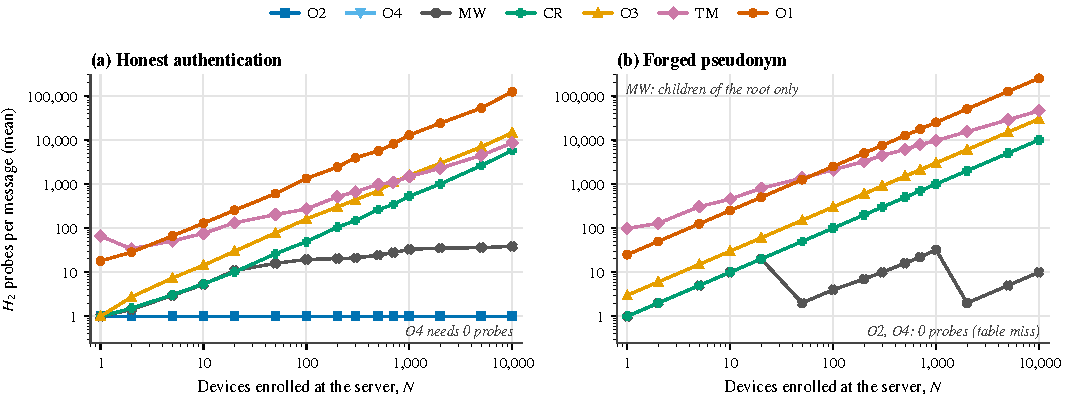
\includegraphics[width=\textwidth]{figures/fig_probes.pdf}
\caption{Probes per message at one server, measured on the implementation (log--log): (a) honest authentication, (b) a forged, random pseudonym}
\label{fig:probes}
\end{figure}

\subsection*{Session latency and storage in the network model}
Table~\ref{tab:ranked} ranks the strategies by mean session latency at $N=1000$ with 5\% adversaries, from the 960 OMNeT++ runs; their closed-form costs are given in Table~\ref{tab:design}. The \emph{base} column ($N=1$) is the value published in~\cite{base}: 23.68\,ms (Tables~III and~V) and 320 bits (Table~VI). Storage is Table~VI's 320 bits per enrolled device plus the resolution state, averaged over the servers. Figures~\ref{fig:latency} and~\ref{fig:storage} plot the same data.

\begin{table}[H]
\centering
\caption{Strategies ranked by mean session latency at $N=1000$ (5\% adversaries); mean of five seeds}
\label{tab:ranked}
\scriptsize
\setlength{\tabcolsep}{3pt}
\renewcommand{\arraystretch}{1.2}
\begin{tabular}{|c|l|r|r|r|r|r||r|r|r|r|r|}
\hline
 & & \multicolumn{5}{c||}{\textbf{Mean session latency (ms)}} & \multicolumn{5}{c|}{\textbf{Storage per server (KB)}}\\ \hline
\textbf{\#} & \textbf{Strategy} & base & 10 & 100 & 500 & 1000 & base & 10 & 100 & 500 & 1000\\ \hline
1 & O2 Counter + precomputed table & 23.68 & 24.17 & 24.25 & 24.40 & 24.40 & 0.04 & 0.93 & 8.78 & 46.1 & 92.9\\ \hline
2 & O4 Clock + per-epoch table & 23.68 & 23.85 & 23.93 & 24.22 & 24.59 & 0.04 & 0.47 & 4.39 & 23.1 & 46.4\\ \hline
3 & MW Key tree & 23.68 & 24.44 & 27.96 & 30.86 & 31.38 & 0.04 & 0.10 & 0.97 & 5.16 & 10.4\\ \hline
4 & CR Randomized hash lock & 23.68 & 24.44 & 28.86 & 51.71 & 94.89 & 0.04 & 0.10 & 0.95 & 5.02 & 10.1\\ \hline
5 & O3 Clock + linear scan & 23.68 & 24.94 & 38.99 & 176.1 & 1,108 & 0.04 & 0.16 & 1.53 & 8.03 & 16.1\\ \hline
6 & TM Rainbow time--memory trade-off & 23.68 & 38.33 & 516.5 & 5,228 & 12,850 & 0.04 & 2.26 & 10.8 & 36.5 & 59.9\\ \hline
7 & O1 Counter + linear scan & 23.68 & 36.02 & 507.9 & 16,947 & 44,010 & 0.04 & 0.12 & 1.15 & 6.02 & 12.1\\ \hline
\end{tabular}
\end{table}

\begin{figure}[H]
\centering
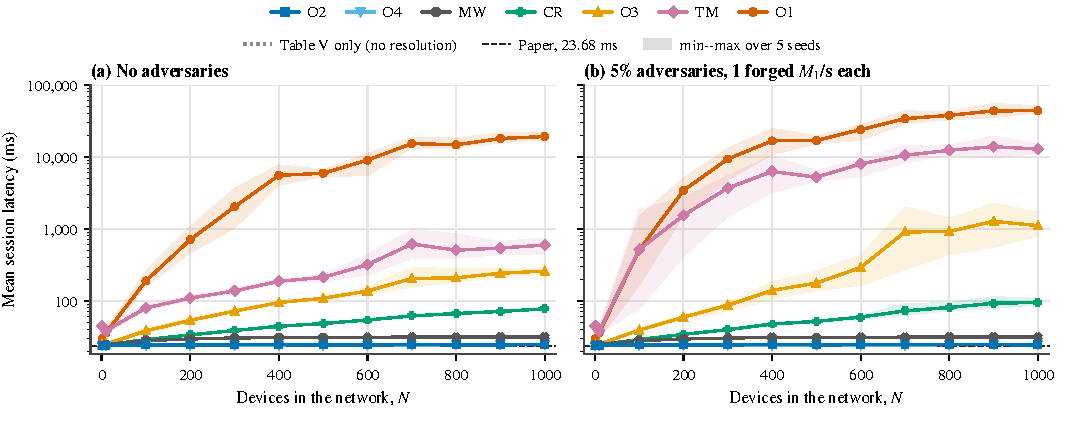
\includegraphics[width=\textwidth]{figures/fig_latency.pdf}
\caption{Mean session latency against network size in the OMNeT++ model (log scale; band: minimum to maximum over five seeds). Dotted: the paper's cost model with no resolution. Dashed: the paper's 23.68\,ms. (a) No adversaries, (b) 5\% adversaries}
\label{fig:latency}
\end{figure}

\begin{figure}[H]
\centering
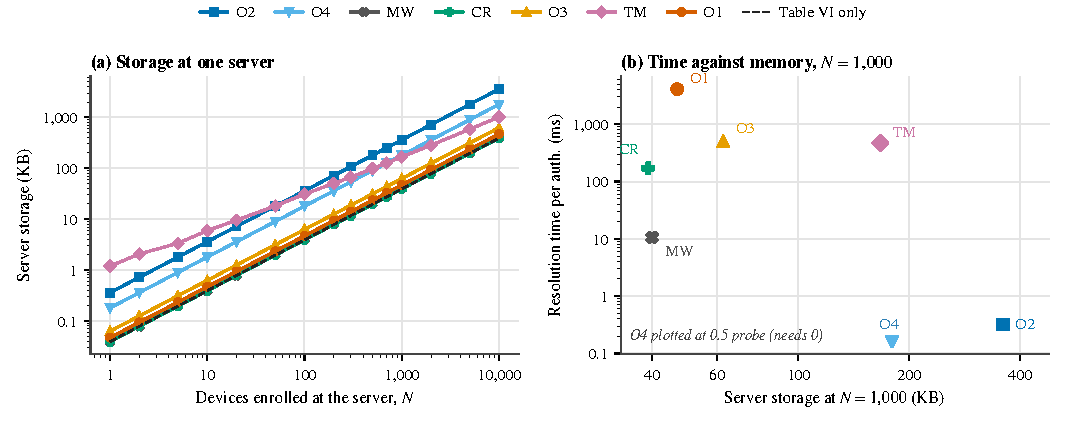
\includegraphics[width=\textwidth]{figures/fig_storage.pdf}
\caption{(a) Server storage at one server (Table~VI's 320 bits per device plus the resolution state); (b) resolution time per authentication ($T_H=0.32$\,ms per probe) against storage at $N=1000$}
\label{fig:storage}
\end{figure}

\subsection*{Desynchronisation}
Table~\ref{tab:desync} is the output of \texttt{desync\_check.py} for counter epochs (re-run for this report; identical to the committed output). An adversary drops $k$ consecutive $M_1$ messages, and the next three honest handshakes are attempted.

\begin{table}[H]
\centering
\caption{Next three honest handshakes after $k$ dropped $M_1$ messages (counter epochs, $F=8$)}
\label{tab:desync}
\small
\begin{tabular}{|c|c|l|}
\hline
\textbf{Dropped $k$} & \textbf{Earlier successful session} & \textbf{Next three honest handshakes}\\ \hline
6 & no / yes & ok, ok, ok\\ \hline
7 & no / yes & ok, ok, ok\\ \hline
8 & no / yes & UnknownPeerError (all three)\\ \hline
9 & no / yes & UnknownPeerError (all three)\\ \hline
12 & no / yes & UnknownPeerError (all three)\\ \hline
\multicolumn{3}{|l|}{Device restart after three successful handshakes (epoch kept in RAM): ReplayDetected}\\ \hline
\end{tabular}
\end{table}

\subsection*{Sensitivity to the assumptions}
The base paper does not fix the adversary share and rate, the authentication window or the enrolment rule, and the per-probe cost $T_H=0.32$\,ms is the paper's constant rather than a measurement on our hardware. Their effect was examined in two ways, without new simulation runs (\texttt{evaluation/resolution/sensitivity.py}, output in \texttt{sensitivity.txt}).

First, the committed OMNeT++ sweep already contains every strategy with and without adversaries (Table~\ref{tab:advcmp}). At $N=1000$ the ranking is identical in both cases.

\begin{table}[H]
\centering
\caption{Simulated mean session latency at $N=1000$ with and without adversaries (ms, mean of five seeds)}
\label{tab:advcmp}
\small
\begin{tabular}{|l|r|r|r|r|r|r|r|}
\hline
 & \textbf{O2} & \textbf{O4} & \textbf{MW} & \textbf{CR} & \textbf{O3} & \textbf{TM} & \textbf{O1}\\ \hline
No adversaries & 24.43 & 24.48 & 31.43 & 77.18 & 258.7 & 595.8 & 19,219\\ \hline
5\% adversaries & 24.40 & 24.59 & 31.38 & 94.89 & 1,108 & 12,850 & 44,010\\ \hline
\end{tabular}
\end{table}

Second, the offered load $\rho$ of the mean server at $N=1000$ was computed from the committed cost model and runs as $\rho=\lambda_h(S+h(n)\,T_H)+\lambda_a f(n)\,T_H$, where $S=11.84$\,ms is the paper's server cost per session, $h$ and $f$ are the measured honest and forged probes, $n=258$ is the mean number of devices enrolled per server, and $\lambda_h$ and $\lambda_a$ are the honest and forged request rates per server (O4 adds its per-epoch extension). A server with $\rho\ge1$ cannot keep up and its queue grows for the whole window. Table~\ref{tab:sens} varies one assumption at a time from the baseline.

\begin{table}[H]
\centering
\caption{Offered load $\rho$ of the mean server at $N=1000$, one assumption varied at a time (baseline: 5\% adversaries at 1\,Hz, 10\,s window, reachable enrolment, $T_H=0.32$\,ms; $\rho\ge1$ means saturated)}
\label{tab:sens}
\small
\begin{tabular}{|l|r|r|r|r|r|r|r|}
\hline
\textbf{Case} & \textbf{O2} & \textbf{O4} & \textbf{MW} & \textbf{CR} & \textbf{O3} & \textbf{TM} & \textbf{O1}\\ \hline
Baseline & 0.02 & 0.03 & 0.04 & 0.19 & 0.52 & 1.68 & 4.16\\ \hline
No adversaries & 0.02 & 0.03 & 0.04 & 0.11 & 0.27 & 0.41 & 2.09\\ \hline
20\% adversaries & 0.02 & 0.03 & 0.05 & 0.44 & 1.26 & 5.47 & 10.3\\ \hline
Adversary rate 2\,Hz & 0.02 & 0.03 & 0.04 & 0.27 & 0.77 & 2.94 & 6.22\\ \hline
Window 5\,s & 0.05 & 0.06 & 0.08 & 0.30 & 0.79 & 2.09 & 6.25\\ \hline
Window 20\,s & 0.01 & 0.02 & 0.02 & 0.14 & 0.38 & 1.47 & 3.11\\ \hline
$T_H=0.16$\,ms & 0.02 & 0.03 & 0.03 & 0.11 & 0.27 & 0.85 & 2.09\\ \hline
$T_H=0.64$\,ms & 0.03 & 0.04 & 0.06 & 0.36 & 1.01 & 3.33 & 8.29\\ \hline
Nearest enrolment & 0.02 & 0.02 & 0.04 & 0.04 & 0.06 & 0.36 & 0.35\\ \hline
\end{tabular}
\end{table}

\subsection*{Formal verification}
Table~\ref{tab:fv} lists the ProVerif~2.05 results (committed logs in \path{evaluation/formal_verification/logs/}); every model finishes in under one second.

\begin{table}[H]
\centering
\caption{ProVerif results}
\label{tab:fv}
\small
\renewcommand{\arraystretch}{1.15}
\begin{tabularx}{\textwidth}{|l|X|l|}
\hline
\textbf{\#} & \textbf{Property} & \textbf{Result}\\ \hline
Q1 & Session key secret (device side), honest pair & true\\ \hline
Q2 & Session key secret (server side), honest device & true\\ \hline
Q3 & Server accepts $M_1$ of honest $V$ $\Rightarrow$ $V$ sent it (non-injective agreement on $V,R,N_i,t$) & true\\ \hline
Q4 & Same, injective (no replay state in the model) & false (replay trace)\\ \hline
Q5 & Device accepts $M_2$ $\Rightarrow$ server derived the same key with the same nonces (injective) & true\\ \hline
FS & Session key secret after a later leak of $k^\star$ & false\\ \hline
U1 & Unlinkability, counter epochs (observational equivalence) & true\\ \hline
U2 & Unlinkability, clock epochs, two sessions in one epoch & fails (equal PIDs)\\ \hline
\end{tabularx}
\end{table}

\section{Result Analysis}
\textbf{Ranking.} The two table strategies, O2 and O4, stay within 1\,ms of the paper's 23.68\,ms up to 1,000 devices (24.40\,ms and 24.59\,ms). O2 needs one probe to slide its window and O4 only its per-epoch extension. Their cost is memory: at 1,000 devices about 93\,KB and 46\,KB per server, against 10\,KB for Table~VI alone. The key tree (MW) is third at 31.4\,ms, but it changes $M_1$, and a compromised device leaks the internal keys it shares with others. The randomized hash lock (CR) needs no extra state, but its latency grows linearly, to 95\,ms. The three scanning strategies over epochs saturate the server: clock scan (O3) at 1.1\,s, the time--memory trade-off at 12.9\,s, and the counter scan (O1) at 44\,s. For O1 and TM, the spread across seeds at $N=1000$ is 10.6\,s and 4.5\,s, because latency depends on how many devices and adversaries share the busiest server.

\textbf{Honest load against forged load.} Without adversaries (Figure~\ref{fig:latency}a), O1 already reaches 19.2\,s at 1,000 devices. Each honest authentication costs about $12.5\,n$ probes, which is 1.0\,s of hashing at the $n\approx258$ devices that a server enrols at $N=1000$, and arrivals outpace this, so the server queue grows. Forged load (Figure~\ref{fig:latency}b) roughly doubles the latency, because every forged pseudonym costs a full miss scan of $Wn$ probes. Such a pseudonym never resolves to a device, so the block-list, which counts failures per device, never sees it. At one server (Figure~\ref{fig:probes}b), a forgery at $n=10{,}000$ costs O1 250,000 probes and TM about 46,000, but costs O2 and O4 nothing, because a table miss needs no hash.

\textbf{Time against memory.} No strategy that keeps the wire format is both fast and small (Figure~\ref{fig:storage}b). O2 buys constant time with $F$ table entries per device (328\,KB in total at $n=1000$), and O4 with $W_t$ entries per device (144\,KB). TM sits in between, at 131\,KB and 1,478 probes, and is dominated here because its table must cover a device's whole lifetime ($m=128$ epochs), not only the current window. MW is the only point that is both small and fast, and it pays with a different $M_1$ and a weaker privacy model.

\textbf{Desynchronisation.} With counter epochs the device advances $t$ every time it builds $M_1$, and the server searches at most $F$ epochs ahead of the last one it accepted. An adversary who drops $F$ consecutive $M_1$ messages therefore locks the device out for good (Table~\ref{tab:desync}, with $F=8$), with or without an earlier successful session. The threshold is the window parameter $F$, which the specification does not fix; a larger $F$ delays the lockout but does not remove it. The lockout holds for O1 and O2, and a unit test checks it for both. A device whose counter lives in RAM is also rejected as a replay after a restart. Message dropping is within the threat model of~\cite{base}. Clock epochs (O3, O4), CR and MW have no per-device counter and cannot desynchronise this way; TM tolerates any number of drops until $t$ reaches the lifetime $m$.

\textbf{Security properties.} The ProVerif results separate the properties that the resolver cannot affect from those it decides. Session-key secrecy (Q1, Q2), agreement on $(V,R,N_i,t)$ (Q3) and injective key agreement for the device (Q5) hold for every correct resolver; Q5 holds because $N_i$ is fresh and bound as associated data of $M_2$. Injective authentication of the device (Q4) fails without replay state: ProVerif finds a trace in which one $M_1$ is accepted twice, so injectivity rests on the epoch window (O1, O2, TM) or the nonce cache (O3, O4), which the specification leaves open. With clock epochs the attacker links two sessions in one epoch by testing their pseudonyms for equality (U2); with counter epochs the equivalence holds (U1). Forward secrecy does not hold, and the base paper does not claim it: a later leak of $k^\star$ reveals $N_i$, $N_j$ and $t$ from the ciphertexts and with them the session key.

\textbf{Sensitivity to the assumptions.} The adversaries change the absolute latencies but not the ranking: without them O1 still reaches 19.2\,s, and O2, O4 and MW move by less than 0.2\,ms (Table~\ref{tab:advcmp}). Across adversary shares of 0 to 20\%, adversary rates of 0.5 to 2\,Hz, windows of 5 to 20\,s and $T_H$ from 0.16 to 0.64\,ms, the order of the strategies by offered load is the order of Table~\ref{tab:ranked}, and O2 and O4 stay below $\rho=0.06$ (Table~\ref{tab:sens}). The absolute figures do depend on the assumptions: O1 saturates the mean server unless $T_H<0.076$\,ms, and with 20\% adversaries or $T_H=0.64$\,ms O3 saturates as well. $\rho$ describes the mean server; the busiest server enrols up to 396 devices, which is why O3 already queues in the simulation at $\rho=0.52$. The enrolment rule matters most. If a server enrols only the devices attached to it ($n\approx20$), no strategy saturates, and CR and MW swap places, as do TM and O1, but O2 and O4 remain first. The window parameters $L$, $F$ and $W_t$ act only through the closed forms of Table~\ref{tab:design}: the lockout threshold equals $F$, and O2's state grows as $40F+8$ bytes per device. The recommendation to precompute therefore holds under every assumption varied, whereas figures such as the 44\,s of O1 hold only under the baseline.

\textbf{What the validation shows and does not show.} Every result rests on a check that can be rerun: the reference vectors and the interoperability run for the implementations, the closed forms for the probe counts, the model without resolution against the paper's 23.68\,ms (23.86\,ms at $N=1$ and 24.07\,ms at $N=1000$, a 0.8 to 1.7\% difference from airtime and quantisation), and ProVerif for the security properties. The offered-load analysis, computed independently of the simulator, also orders the strategies exactly as the simulation does. The checks have limits. The authors' code is not available, so the vectors encode our reading of Section~III of~\cite{base}: they show that both implementations agree with that reading, not that it is the authors' intent. The network model is checked against the paper only where the paper gives a figure, at one device and with no resolution, and its behaviour in saturation has not been compared with another simulator.

\textbf{Comparison with the objectives.} Table~\ref{tab:objectives} relates each objective of Section~1.3 to the evidence obtained.

\begin{table}[H]
\centering
\caption{Objectives and the evidence obtained}
\label{tab:objectives}
\small
\renewcommand{\arraystretch}{1.2}
\begin{tabularx}{\textwidth}{|c|>{\raggedright\arraybackslash}p{0.33\textwidth}|X|}
\hline
\textbf{\#} & \textbf{Objective} & \textbf{Evidence}\\ \hline
1 & Conformant Python and C implementations & 15/15 vector checks in each; 5/5 interoperable handshakes; 125 tests pass\\ \hline
2 & Resolution required; open choices identified & Five-step argument from the specification and the vectors (Section~3.3); two open choices\\ \hline
3 & Seven strategies, measured and validated & Closed forms exact for O1--O4 and CR; honest means within 4 SE; MW within its bound; TM 9 misses in 2,100\\ \hline
4 & Network pricing and ranking & 960 OMNeT++ runs; O2 at 24.4\,ms and O1 at 44\,s at $N=1000$ with 5\% adversaries; ranking unchanged without adversaries and under every assumption varied (Table~\ref{tab:sens})\\ \hline
5 & Failure modes & Forged pseudonyms cost O1 $Wn$ probes and O2/O4 none; lockout after $F$ dropped messages ($F=8$ here)\\ \hline
6 & Formal analysis & Q1--Q3, Q5, U1 true; Q4, FS false; U2 fails\\ \hline
7 & Open release & Code, models, data and logs in the public repository\\ \hline
\end{tabularx}
\end{table}

\section{Limitations}
\begin{itemize}
\item The network model is our model of the paper's stated environment, not the authors' simulation, which is not available. The adversary share and rate, the 10\,s authentication window and the enrolment rule are our assumptions, and the saturated latencies of O1, O3 and TM depend on them.
\item Probes are priced with the paper's constant $T_H=0.32$\,ms; no hardware timings are reported.
\item CR and MW change $M_1$ and are modelled at the resolution level only, not in the full handshake.
\item The TM parameters (six tables, $m=128$) are one point on its trade-off curve, and TM measurements vary between runs because peer secrets are drawn from operating-system randomness.
\item The epoch, window and table parameters are our choices, not the paper's; conformance means agreement with our reading of Section~III.
\item The Python key store is demonstration-grade, re-keying (Eq.~24) is a stub, and coverage (Eqs.~10, 23) is an abstract predicate with no radio model.
\end{itemize}

\section{Observation/Remarks}
\begin{itemize}
\item \textbf{The original implementation was the worst case.} Our first server, written before the resolution study, resolved pseudonyms with a linear scan over a counter window, which is strategy O1. Nothing in the paper warned against it, and it turned out to be the slowest strategy and the one most exposed to forged traffic.
\item \textbf{A precomputed table removes both the scaling and the denial-of-service problem.} Because a table miss needs no hash, forged pseudonyms become free for the server to reject, at a cost of about $40F$ bytes per device.
\item \textbf{The block-list does not protect resolution.} It counts failures per device, but a forged pseudonym never resolves to a device, so the expensive work happens before the block-list can act.
\item \textbf{Specification ambiguities.} Section~II and Section~III of the paper describe different online phases; the implementation follows Section~III, the version covered by the paper's security sketch. The paper also leaves open whether $\mu_1$ covers the clear pseudonym and how $\sigma_2$ is built; these choices are recorded in the assumption register.
\item \textbf{Reproducibility of the measurements.} Re-running the probe sweep for this report reproduced every non-TM row of \texttt{measured.csv} exactly. The TM rows differ, as the repository documents: in our re-run the honest probes per $S^{2/3}$ ranged from 0.42 to 0.67 (0.50 to 0.73 in the committed run) and 7 of 2,100 pseudonyms were missed (9 in the committed run). Regenerating the figures and the ranked table from the committed data reproduced them exactly.
\item \textbf{Independent vectors were essential.} Generating the vectors with code that shares nothing with either implementation fixed the message layout on which the whole gap argument relies, and made the C port's conformance checkable in CI without hardware.
\end{itemize}

\section{Conclusion}
The protocol of~\cite{base} was implemented in Python and, on the device side, in C, and both reproduce the independent reference vectors byte for byte. Seven resolution strategies were implemented and measured, and their probe counts match the closed forms. Under the paper's own constants and network, the choice of resolver decides whether the server stays at the paper's 23.68\,ms per session or saturates at tens of seconds: O2 holds 24.4\,ms at 1,000 devices with 5\% adversaries, while O1 reaches 44\,s. The choice also decides whether forged pseudonyms are free to send and whether $F$ dropped messages ($F=8$ here) lock a device out. Varying the assumptions changes these absolute figures but not the ranking. The formal analysis shows that secrecy and agreement do not depend on the choice, while unlinkability and injective authentication do. All seven objectives were met, within the limitations listed above. The next chapter concludes the report and outlines future work.

% ============================== CHAPTER 5 ==============================
\chapterdivider{5}{CONCLUSION}
\chapter{Conclusion}

\section{Limitations}
\begin{itemize}
\item \textbf{Model, not the authors' simulation.} The OMNeT++ network is our model of the environment stated in Table~II of~\cite{base}; the authors' simulation is not available. The adversary rate, the authentication window and the enrolment rule are our assumptions. The saturated latencies of the scanning strategies depend on them, but the ranking does not (Table~\ref{tab:sens}); apart from the runs with and without adversaries, that analysis uses the offered load of the mean server rather than new simulation runs.
\item \textbf{No hardware timings.} Every probe is priced with the paper's constant $T_H=0.32$\,ms. The ESP8266 port demonstrates that the device side runs on real hardware, but the reported latencies are not measured on it.
\item \textbf{Partial modelling of two strategies.} CR and MW change the first message and are modelled at the resolution level only.
\item \textbf{One point on each trade-off.} The TM parameters (six tables, $m=128$) and the window parameters ($L=16$, $F=8$, $W_t=3$) are single choices; other choices move each strategy along its curve.
\item \textbf{Our reading of the specification.} Epoch semantics, windows and tables are our choices, and conformance means agreement with our reading of Section~III, which only the authors can confirm.
\item \textbf{Symbolic verification only.} The ProVerif results assume perfect primitives and do not include the server's replay state, so injective device authentication (Q4) is checked by test rather than proved.
\item \textbf{Prototype scope.} Devices are static, coverage is an abstract predicate, re-keying is a stub, the key store is demonstration-grade, and side channels are out of scope.
\end{itemize}

\section{Conclusion}
A server cannot authenticate a device that it has not yet identified. In the two-message protocol of Al-Rasheed et al.~\cite{base}, that identification, pseudonym resolution, is a required step with no specification and no cost in the model. This project showed from the specification alone that every correct server must perform it, implemented the protocol in Python and on the device side in C with byte-for-byte conformance to independent vectors, and compared seven ways of filling the gap under the paper's own constants and network.

The choice turned out to decide the protocol's practical behaviour. With a precomputed table (O2) the server stays within 1\,ms of the published 23.68\,ms per session at 1,000 devices and rejects forged pseudonyms for free, at a memory cost of tens of kilobytes per server. With the on-demand counter scan that the specification suggests (O1), the session latency reaches about 44\,s at the same scale with 5\% adversaries, forged pseudonyms are an effective denial-of-service attack that the block-list never sees, and an attacker who drops $F$ consecutive messages ($F=8$ in our configuration) locks a device out for good. This ranking holds under every assumption we varied, although the size of the slowdown depends on them. Clock epochs avoid the lockout but make sessions in one epoch linkable. The formal analysis shows that the protocol's secrecy and agreement properties do not depend on the choice, whereas unlinkability and injective authentication do, and that the protocol has no forward secrecy.

All seven objectives of the project were achieved. The practical recommendation is that a deployment with counter epochs should precompute (O2) and add a resynchronisation path, that a deployment with clocks can use O4 if it accepts linkability within an epoch and keeps a nonce cache, and that the specification should state the epoch semantics, the resolution method and the replay state, and add a resolution term to its cost model. Precomputed tables, the oldest answer from RFID private identification, keep the protocol's cost claim intact.

\section{Future Scope}
\begin{itemize}
\item \textbf{Stateful verification.} Prove injective device authentication with the replay window included, for example in Tamarin, which supports mutable state.
\item \textbf{Hardware measurements.} Measure resolution and handshake times on the ESP8266 and on a server-class machine, and replace the paper's $T_H$ constant with measured values.
\item \textbf{Resynchronisation.} Design and verify a recovery path for counter epochs after the lockout, and study the trade-off between a larger forward window $F$ and table size.
\item \textbf{Full handshakes for CR and MW.} Integrate the strategies that change $M_1$ into the full exchange and the simulator, and quantify MW's privacy loss under device compromise.
\item \textbf{Broader parameter sweeps.} Explore the TM trade-off curve, epoch lengths for O4, adversary rates, mobility and hand-off.
\item \textbf{Re-keying and forward secrecy.} Implement the TA-assisted re-keying of Eq.~24 and evaluate extensions that add forward secrecy.
\item \textbf{Other protocols.} Apply the same method, i.e.\ derive the resolution step from the specification, measure it, and price it under the paper's own constants, to other pseudonym-based IoT authentication schemes.
\end{itemize}

% ============================== REFERENCES ==============================
\clearpage
\phantomsection
\addcontentsline{toc}{chapter}{References}
\renewcommand{\bibname}{References}
\begin{thebibliography}{99}
\bibitem{base} A. Al-Rasheed, R. Khan, A. Ahmad, A. Saeed, F. Alturise and S. Alkhalaf, ``A low-cost hybrid elliptic curve cryptography authentication protocol for trustworthy Internet of Things communication,'' \emph{IEEE Trans. Consum. Electron.}, vol.~72, no.~2, pp.~4483--4491, May 2026, doi:10.1109/TCE.2026.3662053.
\bibitem{weis} S. A. Weis, S. E. Sarma, R. L. Rivest and D. W. Engels, ``Security and privacy aspects of low-cost radio frequency identification systems,'' in \emph{Security in Pervasive Computing (SPC 2003)}, LNCS 2802. Springer, 2004, pp.~201--212.
\bibitem{ohkubo} M. Ohkubo, K. Suzuki and S. Kinoshita, ``Cryptographic approach to `privacy-friendly' tags,'' in \emph{RFID Privacy Workshop}, MIT, Cambridge, MA, USA, Nov. 2003.
\bibitem{molnar} D. Molnar and D. Wagner, ``Privacy and security in library RFID: Issues, practices, and architectures,'' in \emph{Proc. 11th ACM Conf. Computer and Communications Security (CCS)}, 2004, pp.~210--219.
\bibitem{avoine05} G. Avoine and P. Oechslin, ``A scalable and provably secure hash-based RFID protocol,'' in \emph{Proc. 3rd IEEE Int. Conf. Pervasive Computing and Communications Workshops (PerCom Workshops)}, 2005, pp.~110--114.
\bibitem{ado05} G. Avoine, E. Dysli and P. Oechslin, ``Reducing time complexity in RFID systems,'' in \emph{Selected Areas in Cryptography (SAC 2005)}, LNCS 3897. Springer, 2006, pp.~291--306.
\bibitem{tsudik} G. Tsudik, ``YA-TRAP: Yet another trivial RFID authentication protocol,'' in \emph{Proc. 4th IEEE Int. Conf. Pervasive Computing and Communications Workshops (PerCom Workshops)}, 2006, pp.~640--643.
\bibitem{hellman} M. E. Hellman, ``A cryptanalytic time-memory trade-off,'' \emph{IEEE Trans. Inf. Theory}, vol.~26, no.~4, pp.~401--406, 1980.
\bibitem{oechslin} P. Oechslin, ``Making a faster cryptanalytic time-memory trade-off,'' in \emph{Advances in Cryptology -- CRYPTO 2003}, LNCS 2729. Springer, 2003, pp.~617--630.
\bibitem{omnet} A. Varga and R. Hornig, ``An overview of the OMNeT++ simulation environment,'' in \emph{Proc. SIMUTools}, 2008.
\bibitem{hkdf} H. Krawczyk and P. Eronen, ``HMAC-based extract-and-expand key derivation function (HKDF),'' RFC 5869, 2010.
\bibitem{fips180} National Institute of Standards and Technology, ``Secure hash standard (SHS),'' FIPS PUB 180-4, 2015.
\bibitem{gcm} M. Dworkin, ``Recommendation for block cipher modes of operation: Galois/Counter Mode (GCM),'' NIST SP 800-38D, 2007.
\bibitem{proverif} B. Blanchet, ``Modeling and verifying security protocols with the applied pi calculus and ProVerif,'' \emph{Foundations and Trends in Privacy and Security}, vol.~1, no.~1--2, pp.~1--135, 2016.
\bibitem{blanchet08} B. Blanchet, M. Abadi and C. Fournet, ``Automated verification of selected equivalences for security protocols,'' \emph{J. Log. Algebr. Program.}, vol.~75, no.~1, pp.~3--51, 2008.
\bibitem{arapinis} M. Arapinis, T. Chothia, E. Ritter and M. Ryan, ``Analysing unlinkability and anonymity using the applied pi calculus,'' in \emph{Proc. 23rd IEEE Computer Security Foundations Symp. (CSF)}, 2010, pp.~107--121.
\bibitem{repo} J. Kerkar, C. Kelkar, C. Poornamath, Y. Kolekar and S. Sondur, ``hybrid-ecc-iot-auth: Implementation, models and data for pseudonym resolution in two-message IoT authentication,'' 2026. [Online]. Available: \url{https://github.com/jaykerkar0405/hybrid-ecc-iot-auth}
\bibitem{apple} Apple, ``MacBook Pro (14-inch, 2023) -- Tech Specs,'' Apple Support. [Online]. Available: \url{https://support.apple.com/en-am/111340}
\end{thebibliography}

% ============================== APPENDIX ==============================
\clearpage
\chapter*{Appendix}
\addcontentsline{toc}{chapter}{Appendix}

\section*{A.I. Publication Details}
\addcontentsline{toc}{section}{A.I. Publication Details}
\textbf{Paper:} J.~Kerkar, C.~Kelkar, C.~Poornamath, Y.~Kolekar and S.~Sondur, ``Pseudonym Resolution and Formal Verification of an Unlinkable Two-Message IoT Authentication Protocol,'' 2026. Department of Information Technology, Vivekanand Education Society's Institute of Technology, Mumbai. Source and PDF: \texttt{paper/} in the project repository~\cite{repo}.

\textbf{Status:} Publication in progress. Venue, submission and acceptance details will be added when available.

\subsection*{Camera Ready / Published Paper}
\begin{center}
\fbox{\parbox{0.88\textwidth}{\centering\vspace{12pt}
Camera-ready / published paper and presentation certificate\\[6pt]
\textit{Reserved for the final documents when available.}\vspace{12pt}}}
\end{center}

\subsection*{Plagiarism report}
The project paper was checked for similarity using Turnitin (Submission ID 3089310696, 14~November 2026). The overall similarity index is \textbf{3\%}, made up of 2\% internet sources, 1\% publications and 1\% student papers. The matched sources are listed in the report reproduced on the following pages.

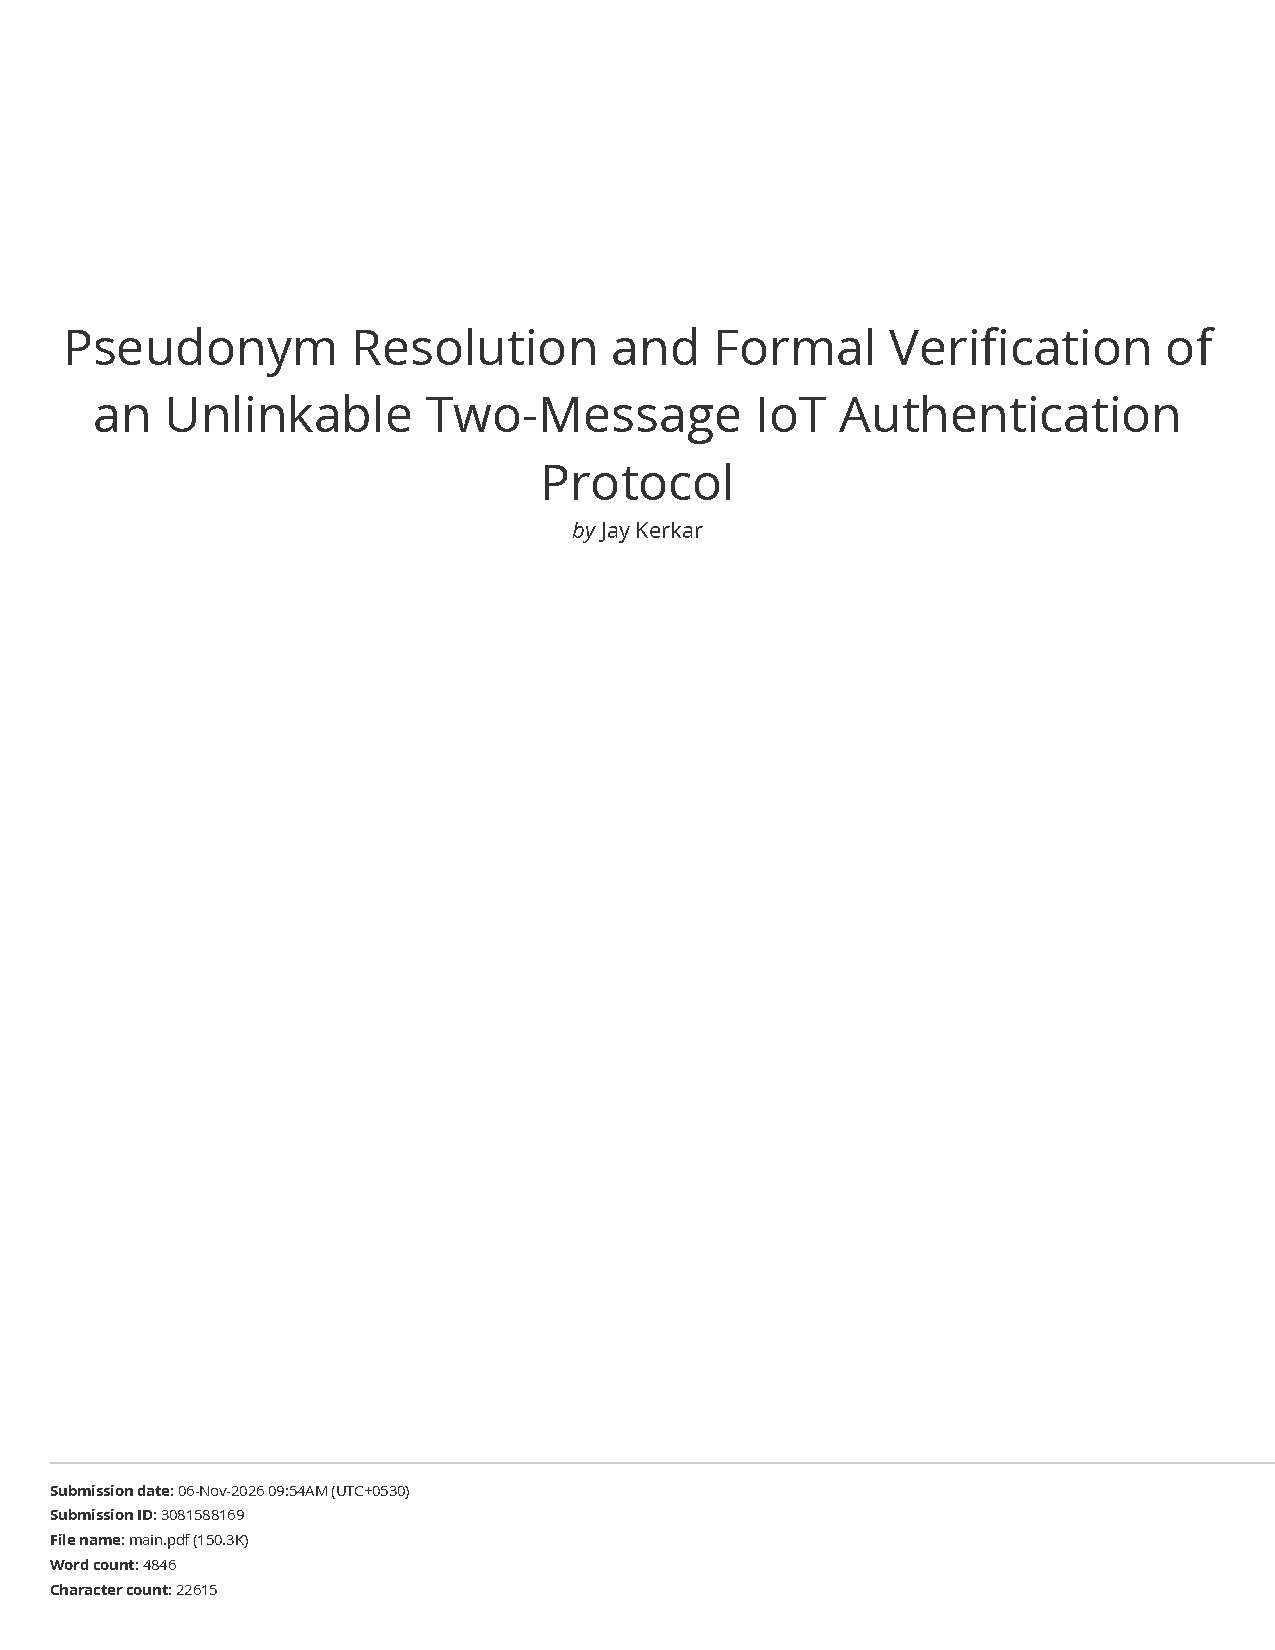
\includepdf[pages=-,scale=0.86,pagecommand={\thispagestyle{bb}}]{reports/plagiarism_report.pdf}

\subsection*{AI writing detection report}
The same paper was also checked with Turnitin's AI writing detection (Submission ID \texttt{trn:oid:::1:3711052702}, 14~November 2026). The report shows no AI-writing score, since scores below the 20\% threshold are not surfaced by the tool. The report is reproduced on the following pages.

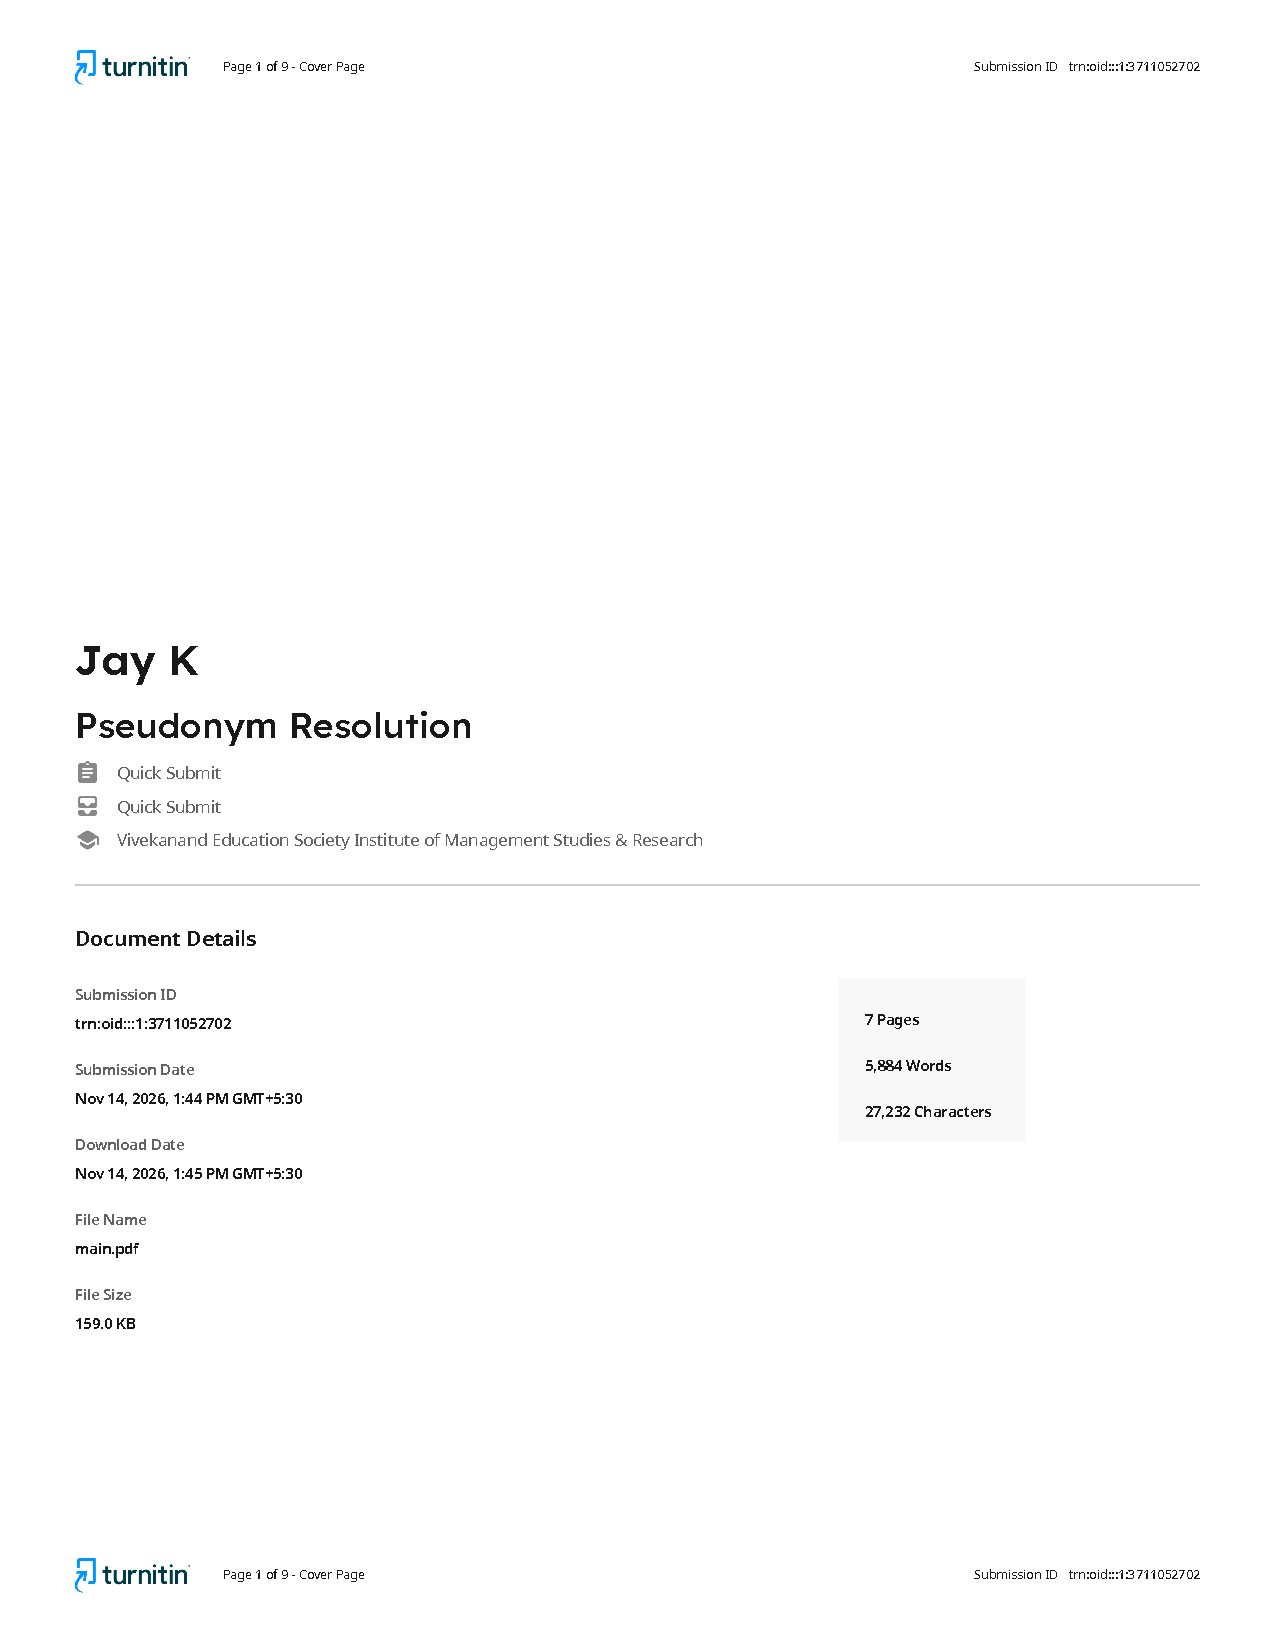
\includepdf[pages=-,scale=0.86,pagecommand={\thispagestyle{bb}}]{reports/ai_detection_report.pdf}

\section*{A.II. IPR: Copyright/Patent/etc. (if granted)}
\addcontentsline{toc}{section}{A.II. IPR: Copyright/Patent/etc.}
The copyright registration application for the project's codebase is being prepared. Application and registration details will be added when available. The software is released under the Apache License~2.0, copyright 2026 Jay Kerkar, Chaitanya Kelkar, Chirag Poornamath, Yash Kolekar and Shanta Sondur.


\end{document}
